\documentclass[a4paper]{article}

\usepackage[english]{babel}
\usepackage[utf8]{inputenc}
\usepackage{amsmath}
\usepackage{graphicx}
\usepackage[colorinlistoftodos]{todonotes}
\usepackage{comment}
\usepackage{float}
\usepackage{placeins}
\usepackage{textcomp}
\usepackage{hyperref}

\title{MPRA Protocol}

\begin{document}
\maketitle

\newpage
\tableofcontents
\newpage

\section{Introduction}
	
    \subsection{Method Overview}
    	\begin{figure}[H]
			\centering
			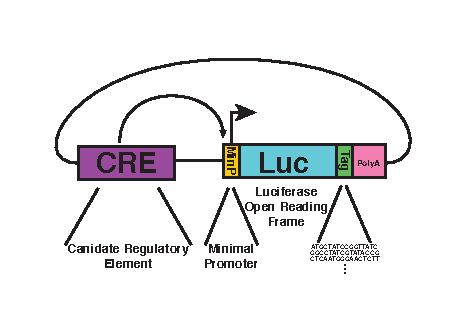
\includegraphics[width=1.0\textwidth]{MPRA_Basic_Fig.pdf}
			\label{fig:Mechanism}
			\caption{Mechanism of Enhancer Interrogation}
        \end{figure}
        \begin{itemize}
                
            \item The MPRA assay relies on measuring candidate enhancers through their transcriptional capacities in parallel. A Candidate Response Element is cloned into a 5' orientation to a MinP driven ORF with a 16 random base pair tag between the ORF and Poly-A tail. Utilizing the proportion of counts assigned to an individual transcript relative to that of the template DNA activity is measured as a fold enrichment.
                              
    	\end{itemize}

	\subsection{Library Construction Overview}
    	\begin{figure}[H]
			\centering
			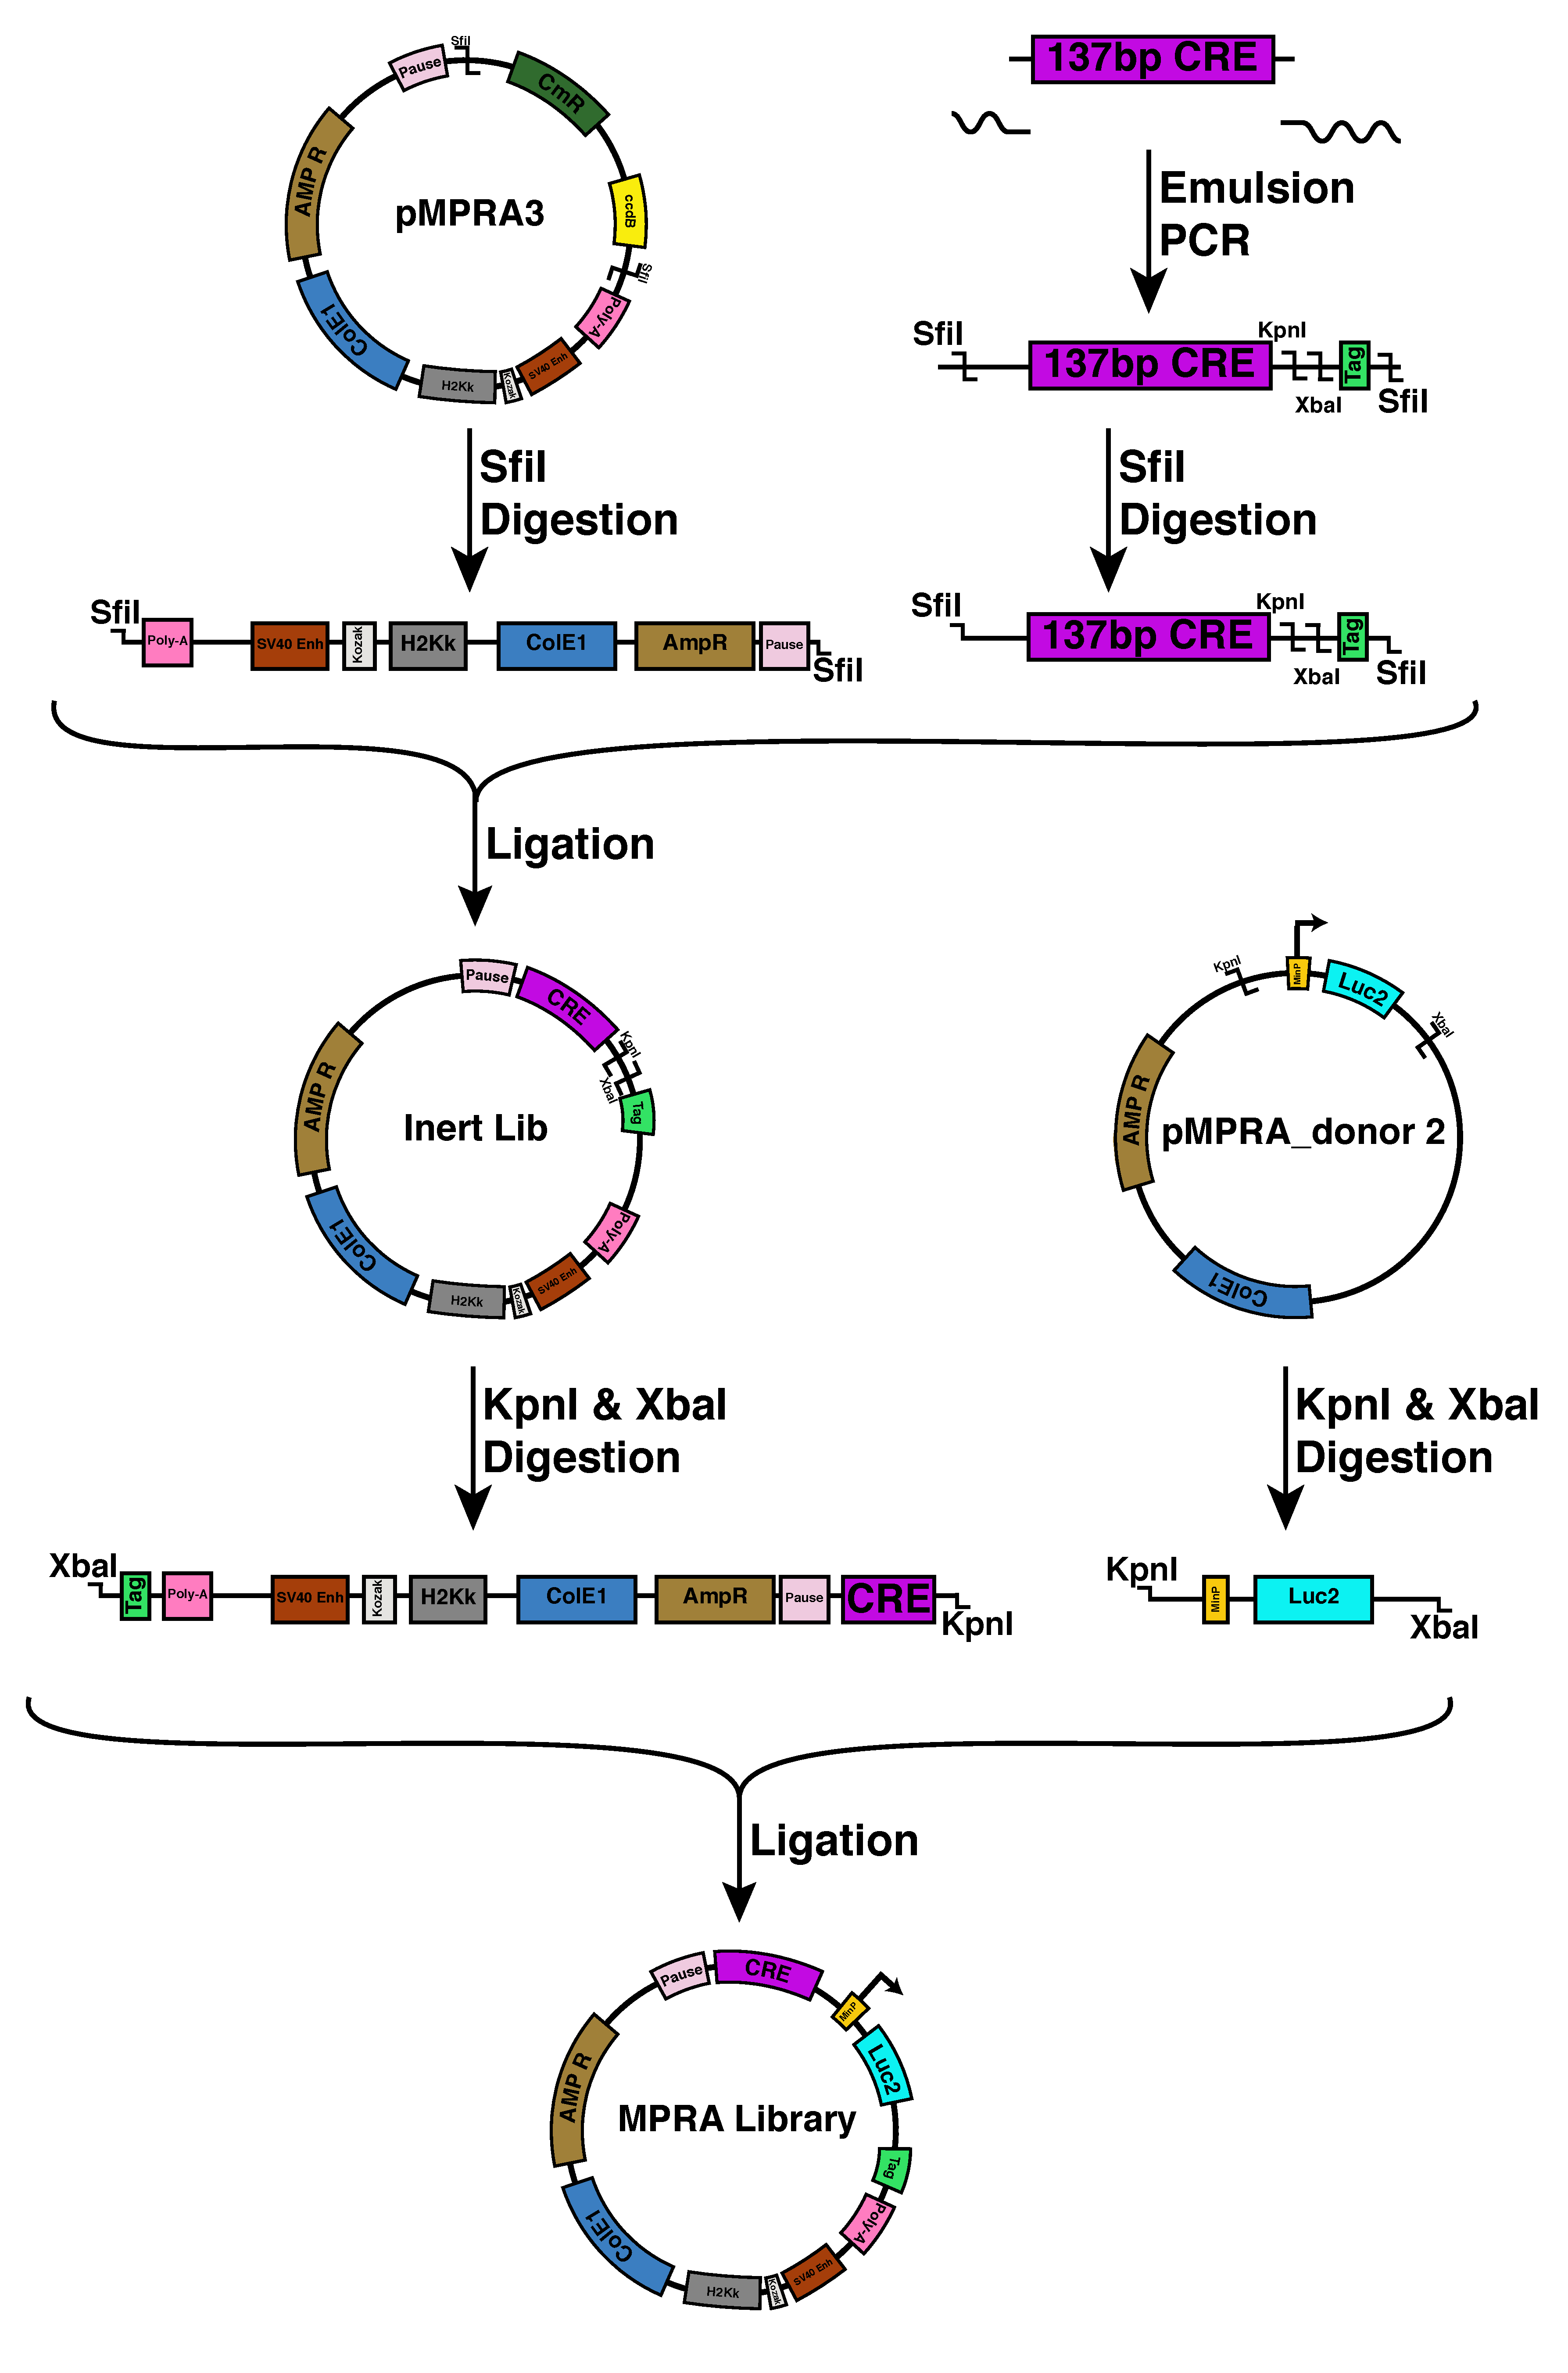
\includegraphics[width=.90\textwidth]{MPRA_LibConstruction.pdf}
			\label{fig:Construction}
			\caption{MPRA Library Construction}
        \end{figure}
        \begin{itemize}
                
            \item The basic schematic of MPRA Library construction above includes an emulsion PCR tailing reaction (table \ref{Emulsion}) and two cloning steps to create a competent library containing an active ORF driven by MinP.
                              
    	\end{itemize}

	\subsection{Emulsion PCR Overview}
    	\begin{figure}[H]
			\centering
			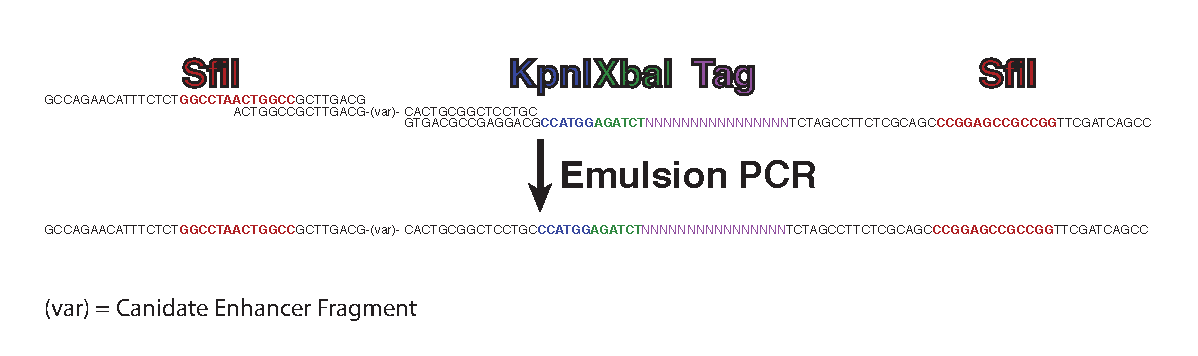
\includegraphics[width=1.0\textwidth]{Sequence_Emulsion_PCR.pdf}
			\label{fig:Emulsion}
			\caption{Tailing Emulsion PCR}
        \end{figure}
        \begin{itemize}
                
            \item The SwiI cloning arms are added to the distal ends to clone into the MPRA backbone vector, while the KpnI and XbaI sites lie in between the candidate enhancer and tag sequence. These sites are used to directionally clone in our Promoter-ORF complex. 
                              
    	\end{itemize}

\section{Library Design}
	\subsection{Fragments} 
    	\begin{itemize}
                
            \item Fragment size is limited by sequencing capacity. The maximum insert size is the maximum synthesis length minus 30 base pairs to account for incorporation of flanking amplification primers. 
                              
    	\end{itemize}
	
    \subsection{Library Primers} 
    	\begin{itemize}
            
            \item First set of primers are un-tailed \\
            Forward: 5' - GCCAGAACATTTCTCT - 3'\\
            Reverse:   5' - GCAGGAGCCGCAGTG - 3'
           
            \item Second set primers utilize tails to add restriction sites and tags to synthesized fragments.
            
            \item The Forward primer adds SwiI (GGCCNNNNNGGCC) cloning site:\\\\
            5' - GCCAGAACATTTCTCT\textbf{GGCCTAACTGGCC}GCTTGACG - 3'
           \item The Reverse primer adds SwiI (GGCCNNNNNGGCC), KpnI(CCATGG), XbaI(AGATCT), and a 16bp tag sequence:\\

				\begin{table}[h]
                    \centering
 					\begin{tabular}{c}
									 	\tiny{CCGACTAGCTT\textbf{GGCCGCCGAGGCC}CGACGCTCTTCCGATCTNNNNNNNNNNNNNNNN\textbf{TCTAGA}\textbf{GGTACC}GCAGGAGCCGCAGTG}          
        			\end{tabular}  
       			 \end{table}
   
		   \item \normalsize{The Reverse primer tag sequences are made by IDT and each \textbf{N} base pair is hand mixed with all nucleotides having an equal proportion of incorporation. The resulting Primer library is purified via HPLC (PAGE has low yield and could skew representation, standard desalting would allow truncated primer products to contaminate primer pool).}

    	\end{itemize}	

\section{Library QC and Preliminary Amplification}    
    \subsection{Single Reaction} 
    	\begin{itemize}
                	
            \item \textbf{Small Cycle qPCR Library Amplification}
          
            \item Observe library amplification with flourescent SYBR Green qPCR reporting on every cycle
            \end{itemize}
        
        	\begin{figure}[H]
				\centering
				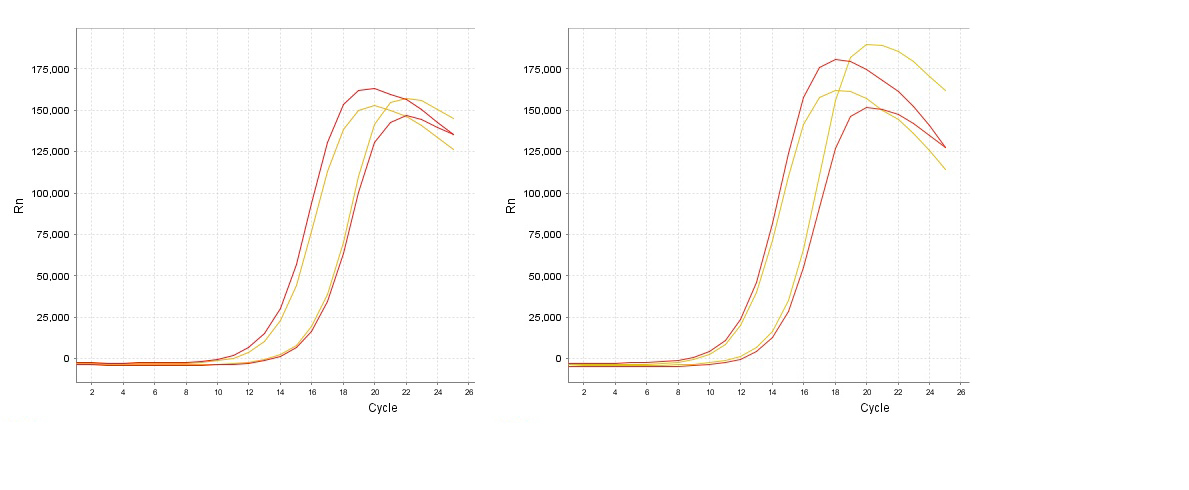
\includegraphics[width=1.0\textwidth]{2016_04_19_PremlimAMPs.jpg}
				\label{fig:Initial qPCR Library Amplification}
				\caption{Initial qPCR Library Amplification Left: Human, Right: Chimp}
		
        	\end{figure}
        	\begin{itemize}

			\item \textbf{PCR Mix:}
          \end{itemize}
         \FloatBarrier
         \begin{table}[H]
			\centering
			\begin{tabular}{l|r|r}
					Reagent 									& 	Volume 				& 	30x 		\\\hline
					2x NEB Master Mix 							& 	10\textmu L 		& 	300\textmu L		\\
					Water 										& 	6.55\textmu L		& 	196.5\textmu L		\\
                    Fwd + Rev Primers (10\textmu mol/\textmu L)	& 	1.25\textmu L		& 	37.5\textmu L		\\
                    10x SYBR Green 								& 	1.2\textmu L		& 	-\textmu L			\\
                    DNA 1:10 dilution							& 	1\textmu L			& 	-\textmu L	\\\hline
                    Final Volume 								& 	20\textmu L			& 	600\textmu L		\\
				\end{tabular}
           		\caption{\label{qPCR}Initial Library PCR.}
        \end{table}     
        \begin{itemize}
			
            \item Pipette out 17.8\textmu L into 7 wells on qPCR plate. 
        	
            \item Add SYBR green and DNA to 5 wells (Fluorescent Reporter Wells)
           	
            \item Add SYBR green and Water in place of DNA to 2 wells (Control Wells)

			\item Add water instead of SYBR green and and DNA to the 23 reaction Master Mix
            
        	\item Pipette 20 wells to collect for purification 

           	\item \textbf{PCR Conditions:}
            	\end{itemize}
         \FloatBarrier
         \begin{table}[H]
			\centering
			\begin{tabular}{l|r|r|l|r}
				Stage 	& 	Temperature	&	Time	&	Cycles		\\\hline
				Stage 1	&	98C			&	30 Sec	&	1 Cycle		\\\hline
						&	98C			&	10 Sec.	&				\\
                Stage 2	&	62C			&	30 Sec.	&	X Cycles	\\
                  		&	72C			&	30 Sec.	&				\\\hline
                Stage 3	&	72C			&	5 Min.	&	1 Cycle		\\
				\end{tabular}
           		\caption{\label{LibqPCRPCR}qPCR Amplification Conditions.}
          \end{table}
            
        \begin{itemize}
        	
            \item Amplification cycles are determined empirically to stop amplification in the log phase
        
        \end{itemize}
        
        	\begin{figure}[H]
				\centering
				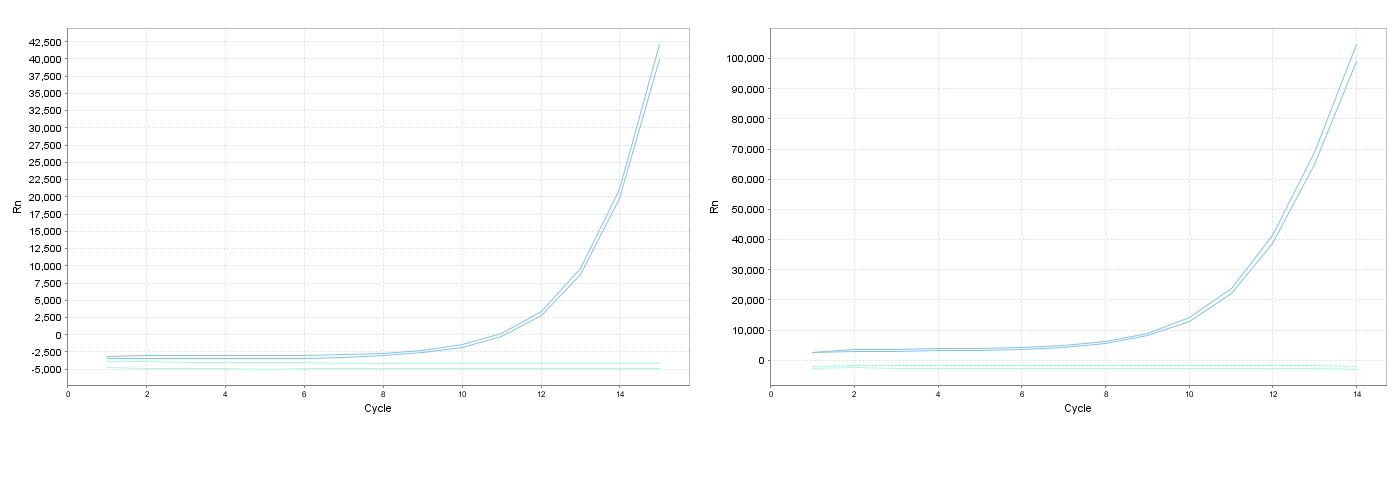
\includegraphics[width=1.0\textwidth]{2016_04_21_Scaled_LibAmp.jpg}
				\label{fig:Scaled qPCR Library Amplification}
				\caption{Left: Human, Right: Chimp}
		
        	\end{figure}
        \begin{itemize}
        
        \item Bead Purified 2x Volume ratio. Elute in 50\textmu L qiagen EB
        
        \end{itemize}
        
\section{Emulsion PCR (CHIMERx: 3600-02)} 
	\subsection{Reaction Mix} 
    	 \begin{itemize}
                	
            \item \textbf{Emulsion:}
          \end{itemize}
         \FloatBarrier
         \begin{table}[H]
			\centering
			\begin{tabular}{l|r|r}
					Reagent 				&	Volume	&	16x 			\\\hline
					Emulsion Component 1 	& 	220		&	3520\textmu L 	\\
					Emulsion Component 3 	& 	60		&	960\textmu L	\\
                    Emulsion Component 2 	& 	20		&	320\textmu L	\\\hline
                    Final Volume & 300\textmu L
				\end{tabular}
           		\caption{\label{Emulsion}Emulsion Component Mixture.}
        \end{table}     
        \begin{itemize}
			
            \item Add components in order, use a wide bore tip for Emulsion Component 2.

            \item Incubate at 4C for 30 minutes on wet ice.
            
            \item \textbf{Aqueous PCR Mix:}
          \end{itemize}
         \FloatBarrier
         \begin{table}[H]
			\centering
			\begin{tabular}{l|r|r}
					Reagent 									& 	Volume 			& 	16x 			\\\hline
					2x NEB Master Mix 							& 	25\textmu L 	& 	400\textmu L		\\
					Water 										& 	19\textmu L		& 	304\textmu L		\\
                    Fwd + Rev Primers (5\textmu mol/\textmu L)	& 	2.5\textmu L	& 	40\textmu L	\\
                    BSA(10mg/mL) 								& 	2\textmu L		& 	32\textmu L		\\
                    DNA 										& 	1\textmu L		& 	16\textmu L		\\
                    q5 Pol 										& 	0.5\textmu L	& 	8\textmu L	\\\hline
                    Final Volume 								& 	50\textmu L		& 	800\textmu L	\\
				\end{tabular}
           		\caption{\label{Emulsion}Emulsion Component Mixture.}
        \end{table}     
        \begin{itemize}
			
            \item Add entire volume to pre-chilled emulsion mix and vortex for 5 minutes on high at 4C.
        	
            \item \textbf{PCR Conditions:}
            
         \end{itemize}
         \FloatBarrier
         \begin{table}[H]
			\centering
			\begin{tabular}{l|r|r|l|r}
				Stage 	& 	Temperature	&	Time	&	Cycles		\\\hline
				Stage 1	&	98C			&	30 Sec	&	1 Cycle		\\\hline
						&	98C			&	20 Sec.	&				\\
                Stage 2	&	72C			&	10 Sec.	&	15 Cycles	\\
                  		&	72C			&	15 Sec.	&				\\\hline
                Stage 3	&	72C			&	5 Min.	&	1 Cycle		\\
				\end{tabular}
           		\caption{\label{LibPCR}PCR Conditions for Library Insert Amplification.}
          \end{table}
            
        \begin{itemize}
        
			\item Each PCR reaction is 50\textmu L per-well.
        	
            \item \textbf{Cleanup:}
            
            \item Pool all reactions and add 1mL of 2-butanol. Vortex thoroughly.
            
            \item Use kit provided spin columns

        \end{itemize}
        
      \subsection{Full Scale Reaction} 
    	 \begin{itemize}
                	
            \item \textbf{Emulsion:}
          \end{itemize}
         \FloatBarrier
         \begin{table}[H]
			\centering
			\begin{tabular}{l|r}
					Reagent 				& 	Volume			\\\hline
					Emulsion Component 1 	& 	3520\textmu L 	\\
					Emulsion Component 3 	& 	960\textmu L	\\
                    Emulsion Component 2 	& 	320\textmu L	\\\hline
                    Final Volume 			& 	300\textmu L
				\end{tabular}
           		\caption{\label{Emulsion}Emulsion Component Mixture.}
        \end{table}     
        \begin{itemize}
			
            \item Add components in order, use a wide bore tip for Emulsion Component 2.

            \item Incubate at 4C for 30 minutes on wet ice.
            
            \item \textbf{Aqueous PCR Mix:}
          \end{itemize}
         \FloatBarrier
         \begin{table}[H]
			\centering
			\begin{tabular}{l|r}
					Reagent 									& 	Volume 			\\\hline
					2x NEB Master Mix 							& 	400\textmu L 	\\
					Water 										& 	319\textmu L	\\
                    Fwd + Rev Primers (5\textmu mol/\textmu L)	& 	40\textmu L		\\
                    BSA(10mg/mL) 								& 	32\textmu L		\\
                    DNA 										& 	1\textmu L		\\
                    q5 Pol 										& 	8\textmu L		\\\hline
                    Final Volume 								& 	800\textmu L
				\end{tabular}
           		\caption{\label{Emulsion}Emulsion Component Mixture.}
        \end{table}     
        \begin{itemize}
			
            \item Add entire volume to pre-chilled emulsion mix and vortex for 5 minutes on high at 4C.
        	
            \item \textbf{PCR Conditions:}
            
         \end{itemize}
         \FloatBarrier
         \begin{table}[H]
			\centering
			\begin{tabular}{l|r|r|l|r}
				Stage 	& 	Temperature	&	Time	&	Cycles		\\\hline
				Stage 1	&	98C			&	30 Sec	&	1 Cycle		\\\hline
						&	98C			&	20 Sec.	&				\\
                Stage 2	&	72C			&	10 Sec.	&	15 Cycles	\\
                  		&	72C			&	15 Sec.	&				\\\hline
                Stage 3	&	72C			&	5Min.	&	1 Cycle		\\
				\end{tabular}
           		\caption{\label{LibPCR}PCR Conditions for Library Insert Amplification.}
          \end{table}
            
        \begin{itemize}
        
			\item Each PCR reaction is 50\textmu L per-well (96 wells total).
        	
            \item \textbf{Cleanup:}
            
            \item Pool all reactions and add 13.7mL of 2-butanol. Vortex thoroughly.
            
            \item Use kit provided spin columns. Condense all volume over 3-4 columns to concentrate eluted library

        \end{itemize}
	
    \subsection{Size Select Library to Remove Slippage Products} 
      	\begin{itemize}
    		\item Slippage on the the random tag sequence causes the production of additional products to arise from the emulsion PCR
        
        \end{itemize}
        
        \begin{figure}[H]
			\centering
			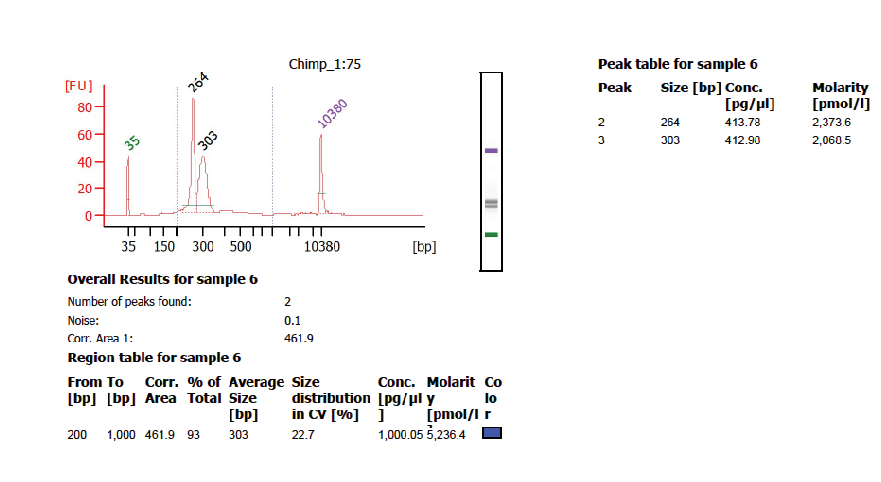
\includegraphics[width=1.0\textwidth]{Size_Issue.pdf}
			\label{fig:Bioanalyzer trace}
			\caption{Extra large molecular weight slippage product \~300bp}
        \end{figure}
        \begin{itemize}
    	
        	\item Libraries were ran in a 2\% Agarose pippen prep gel on Pippin Prep DNA Size Selection System to enrich for the correct 265bp size product.
        
        \end{itemize}
        
        \begin{figure}[H]
			\centering
			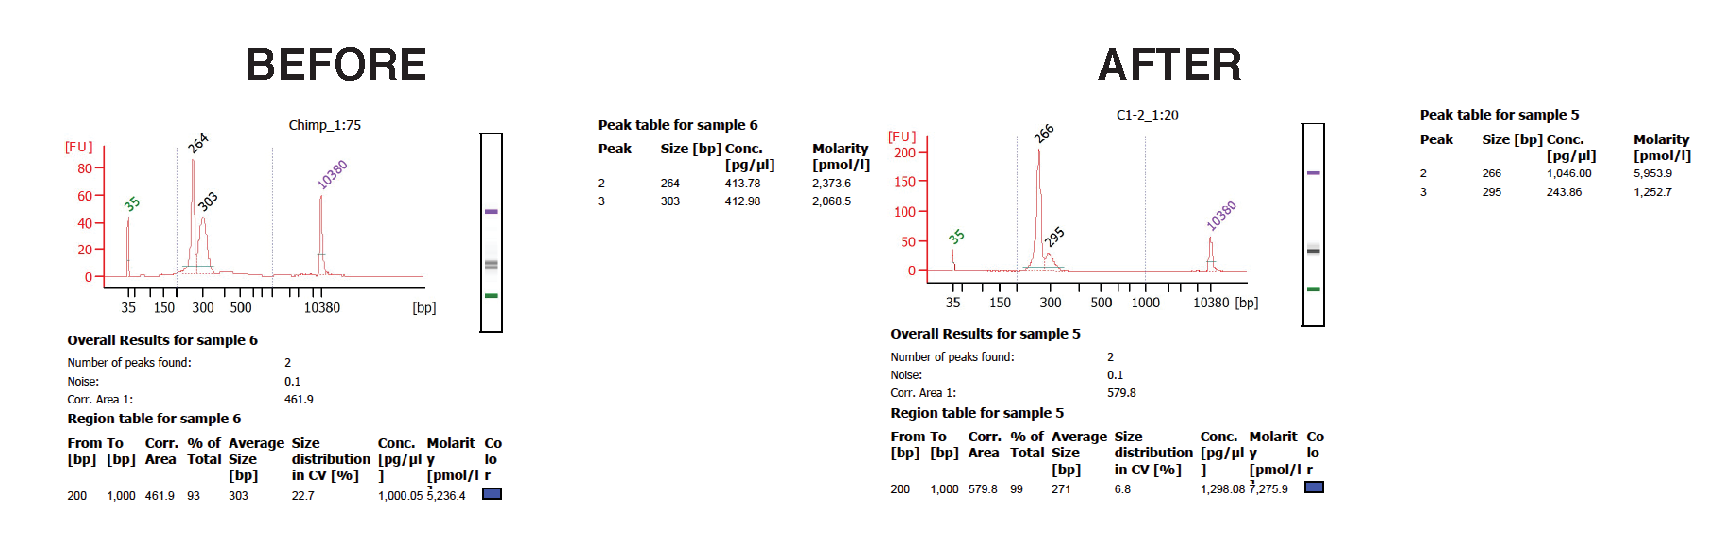
\includegraphics[width=1.0\textwidth]{Size_Select.pdf}
			\label{fig:Size Select}
			\caption{Tailed Libraries Before and After size selection}
        \end{figure}
        
\section{Inert Library Cloning}    
    \subsection{SfiI Digests}
    	
        \begin{itemize}
    	
        	\item Libraries and pMPRA1 vector were digested over night at 37C. Digests were made as described in Table \ref{Digests}.
        
        \end{itemize}
    
    	\FloatBarrier
        \begin{table}[H]
			\centering
			\begin{tabular}{l|r|r|l|r}
                Reagent 		& 	Human Lib	&	Chimp Lib	&	pMPRA1 Vector	\\\hline
				DNA				&	25\textmu L	&	25\textmu L	&	12\textmu L		\\
				Cutsmart Buf	&	3\textmu L	&	3\textmu L	&	2\textmu L		\\
                Water			&	0\textmu L	&	0\textmu L	&	2\textmu L		\\
                SfiI	  		&	2\textmu L	&	2\textmu L	&	4\textmu L		\\\hline
                Final Vol		&	30\textmu L	&	30\textmu L	&	20\textmu L		\\
    		\end{tabular}
          	\caption{\label{Digests}Initial Library Digests.}
        \end{table}
         
        \begin{itemize}
    	
        	\item Add 2\textmu L CIP, 1\textmu L Cutsmart Buffer and 7\textmu L Water to the pMPRA1 vector digest. Incubate at 37C for one hour.
            
            \item Clean up Fragment Library digests with Min Elute columns. Elute in 8\textmu L EB buffer. 
        
        	\item Run out pMPRA1 digest on a 1\% agarose gel. Excise larger backbone band and gel purify. 
            \item \textit{Alternativley you can digest the pMPRA 1 pasmid with SfiI, NcoI, AclI, and XmaI. This yeilds a 2.4Kb band and all other bands are less than 600bp. Use AmpureXP beads to size select and CIP the eluted DNA. This allows you to avoid the gel extraction}
            
             \end{itemize}
        
        \begin{figure}[H]
			\centering
			\includegraphics[width=0.60\textwidth]{pMPRA1_GelExtract.pdf}
			\label{fig:Gel Extract}
			\caption{Gel Extract pMPRA1 Backbone to isolate from insert}
        \end{figure}
        
        \begin{itemize}
        
            \item Purify backbone though second purification with 1X beads. Elute in EB.
            
        \end{itemize}
	
    \subsection{Library Ligation}
    
    	\begin{itemize}
			
            \item Before setting up the ligation reaction confirm that the fragment libraries have been completly digested on both ends by running a bioanalyzer high sensitivity chip on them. 
            
        \end{itemize}
        
        \begin{figure}[H]
			\centering
			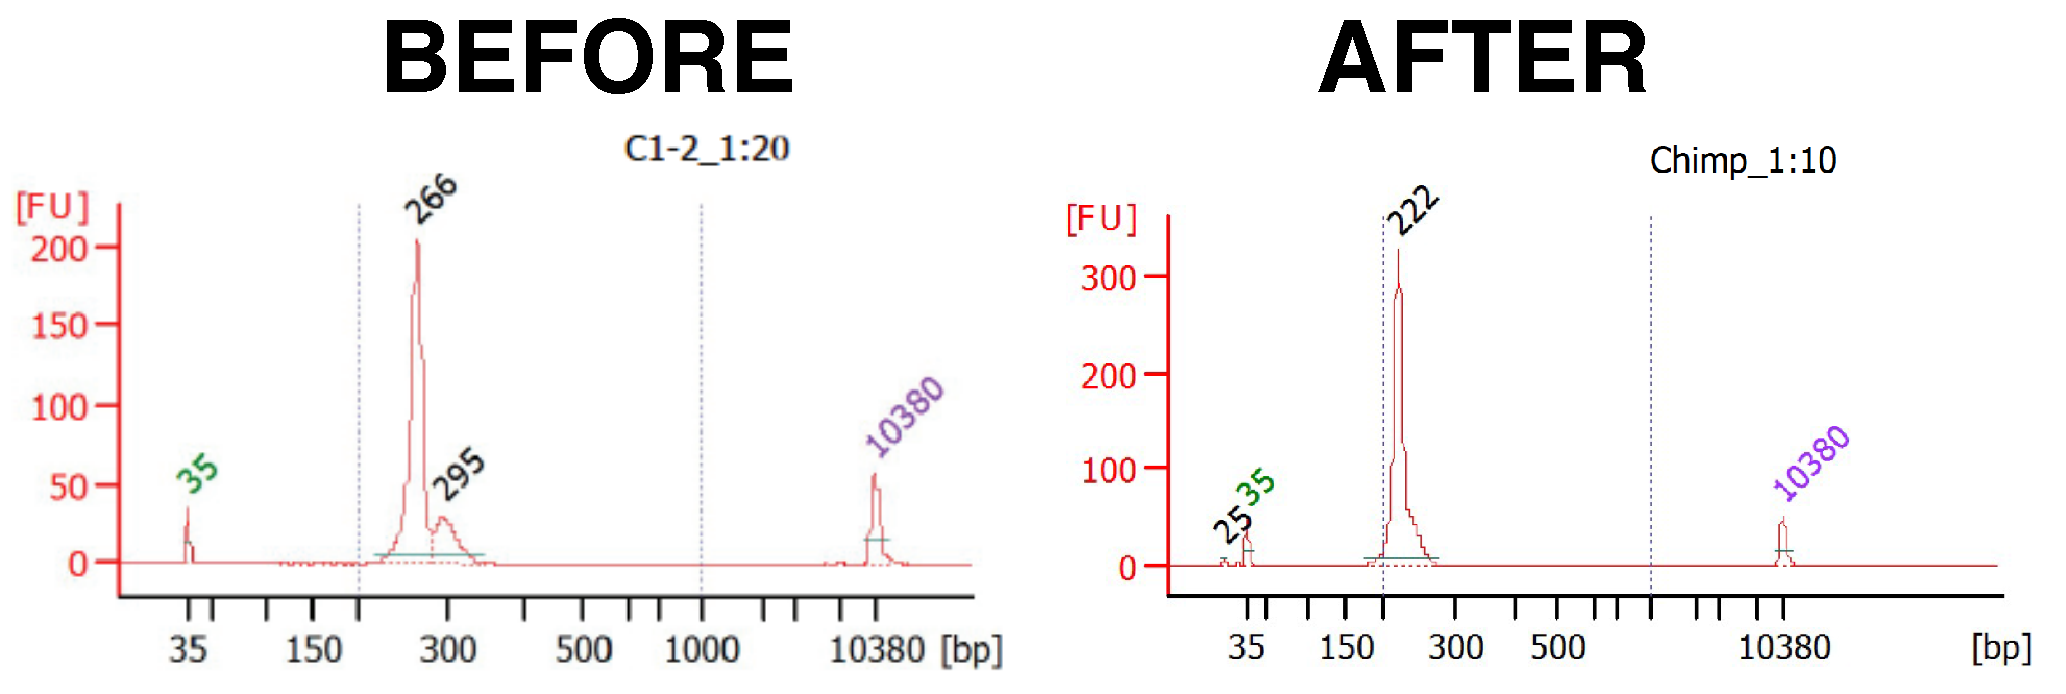
\includegraphics[width=1.0\textwidth]{Frag_Digest.pdf}
			\label{fig:Frag_Digest}
			\caption{The 266bp library fragments should lose \~40 base pairs after digest}
        \end{figure}
        
        \begin{itemize}
        
        \item Ligation reactions are preformed a Fragment to backbone ratio of 3:1. Backbone input mass is 340ng, making this particular library input mass 103ng. 2000 units of ligase is used per-reaction. Ideally each reaction should yield \~5,000,000CFU. Reactions were setup as described in table in Table \ref{Ligations}.
        \end{itemize}
    
    	\FloatBarrier
        \begin{table}[H]
			\centering
			\begin{tabular}{l|r|r|l|r}
            
    Reagent 					& 	Human			&	Chimp			&	Combined	\\\hline
	Water						&	-\textmu L		&	3.48\textmu L	&	-\textmu L		\\
	Fragment Lib				&	-\textmu L		&	5.80\textmu L	&	-\textmu L		\\
	Vector (91.5ng/\textmu L)	&	3.72\textmu L	&	3.72\textmu L	&	7.44\textmu L	\\
    10x Buffer	  				&	2\textmu L		&	2\textmu L		&	4\textmu L		\\
    Ligase (400U/\textmu L)		&	5\textmu L		&	5\textmu L		&	10\textmu L	\\\hline
    Total Volume				&	20\textmu L		&	20\textmu L		&	40\textmu L		\\
    
    		\end{tabular}
          	\caption{\label{Ligations}Initial Library Digests.}
        \end{table}
         
        \begin{itemize}
        
        	\item Ligations incubated for 16 hours at 16C in a thermocycler. 20\textmu L per-tube.
        
        \end{itemize}
               
    \subsection{Library Transformation}
    
    	\begin{itemize}
        
        	\item Ligations should be cleaned up with room temperature AMPure XP beads. Add 20\textmu L beads per-20\textmu L ligation reaction. Incubate 5 minutes. Apply magnet for 5 minutes.
            
            \item Remove supernatant and wash twice with 200\textmu L 80\% ethanol. Air dry for 10-15 minutes and elute in 10uL EB per-20\textmu L ligation reaction. 
            
            \item Label all LB-AMP plates (100ug/mL) plates and place in 37C incubator to pre-warm
            
            \item Label tubes for a tenfold dilution series and fill with recovery media according to the serial dilution table below: 
        
    	\end{itemize}
            \FloatBarrier
            \begin{table}[H]
				\centering
				\begin{tabular}{l|r|l|r|l|r|l|r|l|r|l|r|l|r|l|r}
Dilution		& 	1:10	&	1:100	&	1:1,000	&	1:5,000	&	1:10,000*	&	1:50,000	&	1:100,000*	\\\hline
Recovery Media	&	90\textmu L	&	90\textmu L	&	90\textmu L	&	40\textmu L		&	90\textmu L		&	40\textmu L		&	90\textmu L		\\
Cell Volume		&	10\textmu L	&	10\textmu L	&	10\textmu L	&	10\textmu L		&	10\textmu L		&	10\textmu L		&	10\textmu L		\\                    
				\end{tabular}
           		\caption{\label{PlatingDil}Serial dilution schema for ligation and transformation efficiency.
                	\newline 
                    \textbf{*}\textit{These dilutions are made from the proceeding ten-fold dilution not the half fold dilution}}
           \end{table}
            
       	\begin{itemize}
        
        	\item Place 5 electroporation cuvettes per-20\textmu L recombination reaction and a 1.5mL eppendorf tube on ice for each transformation reaction
            
            \item Thaw cells on watery ice, make sure the water has time to come down to 4C, mix cells by gently flicking the side of the tube. \textbf{DON’T VORTEX}
            
            \item Pipette 20\textmu L of thawed cells into the eppendorf tube on ice with a \textbf{wide bore} pipette tip
        	
            \item Pipette 2\textmu L of DNA into the 20\textmu L of cells and tap tube to mix
            
            \item Incubate on ice for 10min
            
            \item Take 21\textmu L of the cells with a \textbf{wide bore} pipette tips and place in the center of the cuvette. Tap the cuvette gently on the table to get the cells to fall into the bottom and rid the cells of any air bubbles 
 
            \item Place into electroporator arm and ensue that the metal cuvette is dry with a chem-wipe. Be sure not to warm the cuvette with your hand

            \item Electroporate at 200\textohm , 25\textmu Fd, 2.0kV, and immediately place the cuvette back on ice

            \item Place 1mL of \textbf{room temperature} recovery into the cuvette

            \item Use a \textbf{wide bore} 1mL pipette tip to mix the cells once and then remove the cells slowly while rotating the cuvette on its side to ensure the cuvette well is drained. Place the cells into a 15mL falcon tube

            \item Loosely fasten the cap to allow gas exchange and incubate at 37C \& 225RPM for 1hr

			\item Pool all reactions and remove 10\textmu L and dilute the cells according to table \ref{PlatingDil}. Plate two plates with 10\textmu L of each dilution
            
            \item For every transformation, \textbf{seed a range} of 500mL of LB-Amp in 2.5L flasks.  
            
            \item Grow colonies at 37C \& 225RPM for 8–11hr. \textbf{UNTIL OD = 0.95-1.2}
            
            \item Pellet cells at 4500rpm for 15 minutes at 4C
            
        \end{itemize}
    
    \subsection{Plasmid Library Purification} 
    	\begin{itemize}
                	
            \item Plasmid library is purified with HiSpeed Qiagen Maxi kit (12662)
        
    	\end{itemize}    
     
     \subsection{Estimate Complexity and Blend Libraries}
     	\begin{itemize}
     		\item Calculate the concentration of competent transformants utilizing the diluted series of plates equation 
 
			 	\begin{center}
        			$CFU per\mu L  Seeded = \frac{ AvgCFU \times Dilution Factor} {10 \mu L}$
				\end{center}
            
            \item ~80 tags per-canidate enhancer is the target for a 52,000-104,000 element library
            
            \item Therefore for a 52,000 element library:
            	\begin{center}
        			$4,200,000 \approx CFU per\mu L Seeded \times \mu L Seeded$
				\end{center}
            
            \item If one dilution is not within 20\% of your targeted complexity then you can blend libraries togeather to equal the correct complexity. Blending should be done with library \textbf{masses} proportional to the complexity seeded. This allows for roughly equivalent molecular molarity of any given CRE-Tag molecular.
            
		\end{itemize}
     
     \subsection{\label{QC}QC Inert Library} 
    	\begin{itemize}
            
            \item Equation to calculate total number of independent ligated transformants:    	
            
            \begin{center}
        $Total Complexity = CFU \times Dilution Factor \times \frac{Volume of Cells Cultured (\mu L)} {10 \mu L}$
			\end{center}
            
            \item Set up four different restriction digests of the purified inert library as described in table \ref{DigestsQC}.
        
    	\end{itemize}    
        
    	\FloatBarrier
        \begin{table}[H]
			\centering
			\begin{tabular}{l|r|r|l|r|l|r}
            
    Reagent 			& 	SfiI			&	XbaI			&	AfeI		&	NdeI		\\\hline
	Water				&	10\textmu L		&	10\textmu L		&	10\textmu L	&	10\textmu L	\\
	DNA(100ng\textmu L)	&	5\textmu L		&	5\textmu L		&	5\textmu L	&	5\textmu L	\\
	10x Buffer			&	2\textmu L		&	2\textmu L		&	2\textmu L	&	2\textmu L	\\
    SfiI	  			&	3\textmu L		&	-\textmu L		&	-\textmu L	&	-\textmu L	\\
    XbaI	  			&	-\textmu L		&	3\textmu L		&	-\textmu L	&	-\textmu L	\\
    AfeI	  			&	-\textmu L		&	-\textmu L		&	3\textmu L	&	-\textmu L	\\
    NdeI				&	-\textmu L		&	-\textmu L		&	-\textmu L	&	3\textmu L	\\\hline
    Total Volume		&	20\textmu L		&	20\textmu L		&	20\textmu L	&	20\textmu L	\\
    
    		\end{tabular}
          	\caption{\label{DigestsQC}Inert Library Digests.}
        \end{table}
         
        \begin{itemize}
                	
            \item Run out all four digests on a 1\% agarose gel.
        	
            \item If library is correctly constructed it will digest according to figure 10.
            
    	\end{itemize}
        
		\begin{figure}[H]
			\centering
			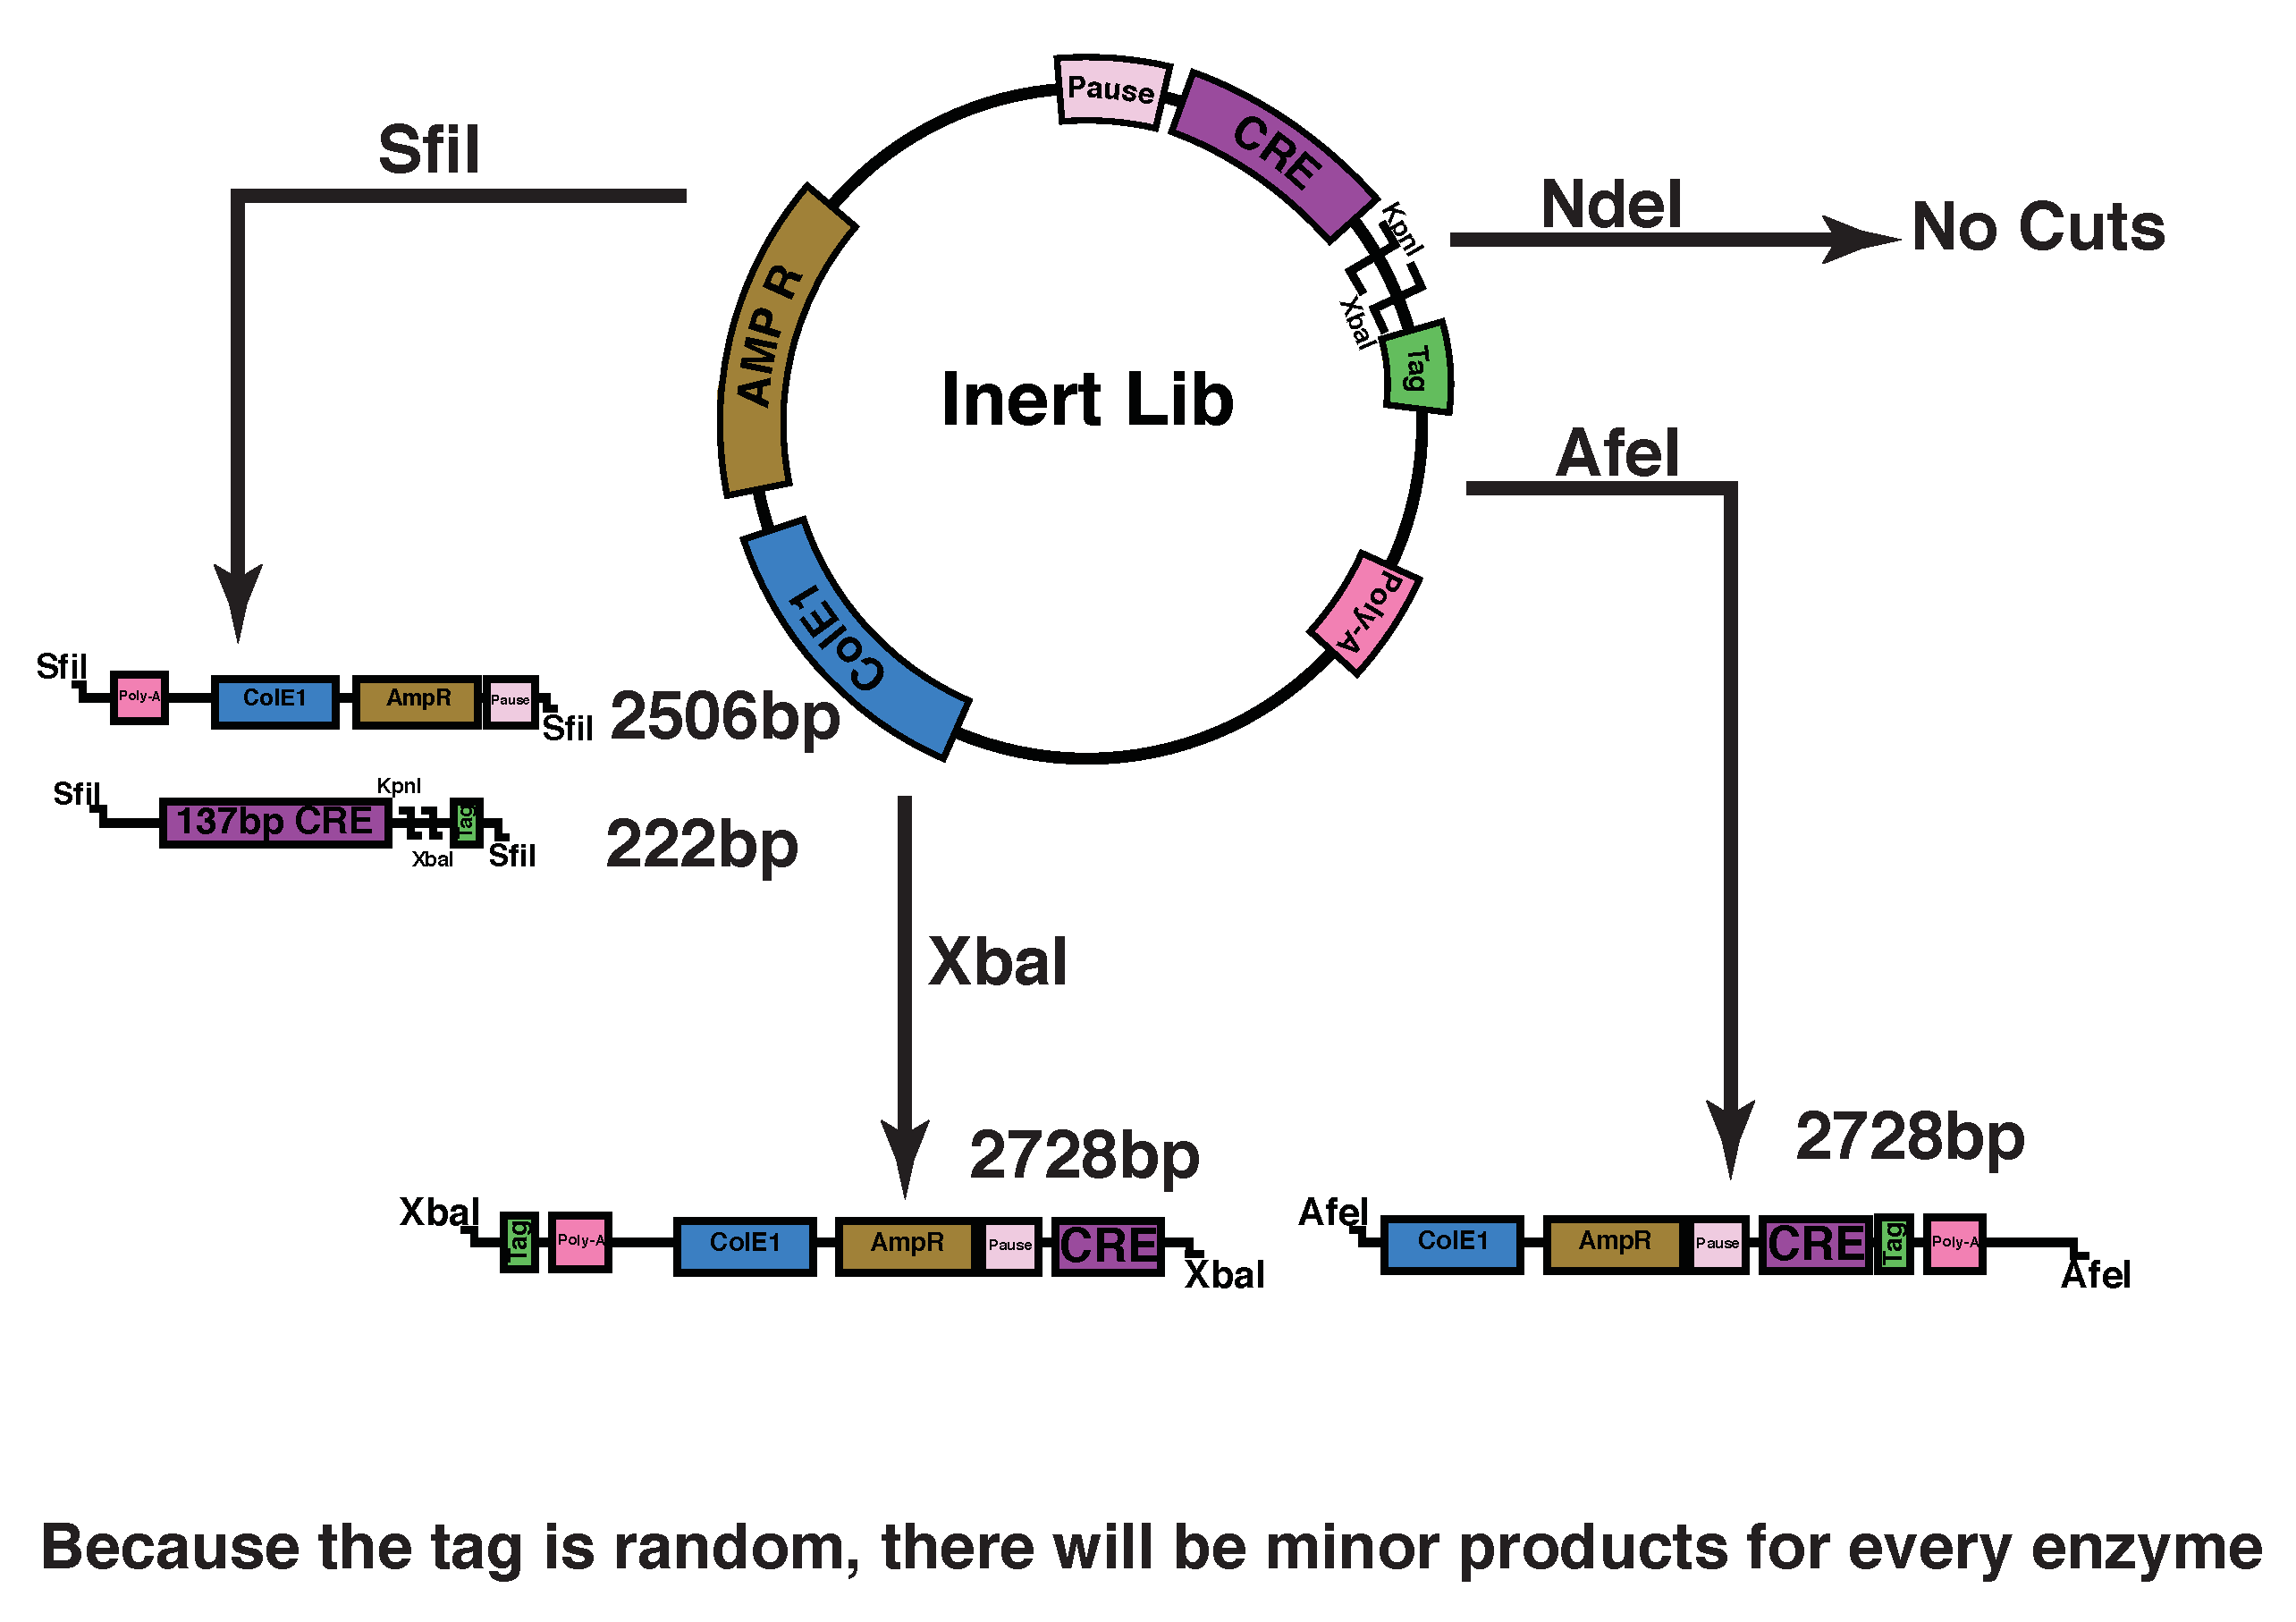
\includegraphics[width=1.0\textwidth]{Inert_Lib_Digest.pdf}
			\label{fig:InertLib_Digest}
			\caption{Library QC Digest schematic}
        \end{figure}
        
        \begin{itemize}
        
        \item Digestion gel should look similar to figure 11.
        
        \end{itemize}
        
        \begin{figure}[H]
			\centering
			\includegraphics[width=0.50\textwidth]{InertLib_Digest_PIC.pdf}
			\label{fig:InertLib_DigestGel}
			\caption{Library QC Digest}
        \end{figure}
        
\section{Library Sequencing}
	\subsection{PCR Amplification Off Inert Library}
    	 	\begin{itemize}
                	
            \item Dilute primers to 100uM, then mix forward and reverse primers to a final working concentration of 10uM
            
            \item Setup PCR reactions as follows:
            
		\end{itemize}
            \FloatBarrier
            \begin{table}[H]
				\centering
				\begin{tabular}{l|r|r}
					Reagent 						& 1x 				& 10x 			\\\hline
					5X Q5 Buffer					& 10\textmu L 		& 100\textmu L	\\
					5X GC Enhancer					& 10\textmu L 		& 100\textmu L	\\
					DMSO							& 2.5\textmu L 		& 25\textmu L	\\
                    Primers (10uM)					& 2.5\textmu L 		& 25\textmu L	\\
                    dNTPs (25uM)					& 0.4\textmu L 		& 4\textmu L	\\
                    Library DNA (3ng/\textmu L)		& 0.5\textmu L 		& 5\textmu L	\\
                    Q5 Polymerase					& 0.5\textmu L 		& 5\textmu L	\\
                    Water							& 22.25\textmu L	& 236\textmu L	\\\hline
                    Final Volume					& 50\textmu L 		& 500\textmu L
				\end{tabular}
           		\caption{\label{LibPCR}Volumes Library PCR Reactions.}
           \end{table}
            
       	\begin{itemize}      
        
        	\item Run 10 PCR reactions under the following conditions:

		\end{itemize}
            \FloatBarrier
            \begin{table}[H]
				\centering
				\begin{tabular}{l|r|r|r}
					Stage 	& 	Temperature	&	Time	&	Cycles		\\\hline
					Stage 1	&	98C			&	30 sec.	&	1 Cycle		\\\hline
							&	98C			&	10 Sec.	&				\\
                    Stage 2	&	68C			&	20 Sec.	&	18 Cycles	\\
                    		&	72C			&	20 Sec.	&				\\\hline
                    Stage 3	&	72C			&	5Min.	&	1 Cycle		\\
				\end{tabular}
           		\caption{\label{LibPCR}PCR Conditions for Library Insert Amplification.}
           \end{table}
            
       	\begin{itemize}          
    	
        \item Pool the 10 PCR reactions and cleanup with 1.4x AMPureXP Beads. Elute in 30\textmu L EB.
        
        \item Check size fraction and concentration in Bioanalyzer 
        
        \end{itemize}
        
    \subsection{dA-Tailing} 
    	 \begin{itemize}
          	\item Combine the following:
            
         \end{itemize}
         \FloatBarrier
         \begin{table}[H]
			\centering
			\begin{tabular}{l|r}
					Reagent 								& Volume 		\\\hline
					End Repaired DNA 						& 42\textmu L 	\\
					10x NEBNext End Repai Reaction Buffer 	& 5\textmu L	\\
                    Klenow Fragment (3' - 5' exo-) 			& 3\textmu L	\\\hline
                    Final Volume 							& 50\textmu L
				\end{tabular}
           		\caption{\label{dA_Tail}dA Tailing Reaction.}
        \end{table}     
        \begin{itemize}      	
        	\item Incubate at 37C for 30 minutes
        	          
            \item Clean up with Qiagen QIAQuick PCR Purification kit. Elute in 25\textmu L EB
        
    	\end{itemize}	
    \subsection{Adaptor Ligation} 
    	 \begin{itemize}
          	\item Combine the following:
            
         	\end{itemize}
         	\FloatBarrier
         	\begin{table}[H]
				\centering
				\begin{tabular}{l|r}
					Reagent 									& Volume 		\\\hline
					dA-Tailed DNA 								& 25\textmu L 	\\
					5x NEBNext Quick Ligation Reaction Buffer 	& 10\textmu L	\\
                    15uM NEBNext Adaptors 						& 10\textmu L	\\
                    Quick T4 DNA Ligase 						& 5\textmu L	\\\hline
                    Final Volume 								& 50\textmu L
				\end{tabular}
           		\caption{\label{AdaptorLigation}Adaptor Ligation Reaction.}
        \end{table}     
        \begin{itemize}      	
        	\item Incubate at 20C for 15 minutes
        	          
            \item Clean up with Qiagen QIAQuick PCR Purification kit. Elute \textbf{twice} in 25\textmu L EB (final volume = 50\textmu L)
        
    	\end{itemize}	    
	  
    \subsection{Indexing PCR Amplification}
    	\begin{itemize}
                	
            \item Dilute PCR primers to a final working concentration of 50uM
            
            \item Setup PCR reactions as follows:
            
		\end{itemize}
            \FloatBarrier
            \begin{table}[H]
				\centering
				\begin{tabular}{l|r|r}
					Reagent 				& 1x 				& 5x 				\\\hline
					2x NEB High Fidelity 	& 12.5\textmu L		& 62.5\textmu L		\\
					Library DNA 			& 1\textmu L 		& 5\textmu L		\\
                    F-Primer (10uM) 		& 1.25\textmu L 	& 6.25\textmu L		\\
                    R-Primer (10uM) 		& 1.25\textmu L 	& 6.25\textmu L		\\
                    Water 					& 9\textmu L 		& 45\textmu L	\\\hline
                    Final Volume 			& 25\textmu L 		& 125\textmu L
				\end{tabular}
           		\caption{\label{LibPCR}Volumes Library PCR Reactions.}
           \end{table}
            
       	\begin{itemize}      
        
        	\item Run 4 PCR reactions under the following conditions:

		\end{itemize}
            \FloatBarrier
            \begin{table}[H]
				\centering
				\begin{tabular}{l|r|r|r}
					Stage 	& 	Temperature	&	Time	&	Cycles		\\\hline
					Stage 1	&	98C			&	30 Sec.	&	1 Cycle		\\\hline
							&	98C			&	10 Sec.	&				\\
                    Stage 2	&	65C			&	30 Sec.	&	10 Cycles	\\
                    		&	72C			&	30 Sec.	&				\\\hline
                    Stage 3	&	72C			&	5 Min.	&	1 Cycle		\\
				\end{tabular}
           		\caption{\label{LibPCR}PCR Conditions for Library Insert Amplification.}
           \end{table}
            
       	\begin{itemize}          
    	
        \item Pool the 4 PCR reactions and cleanup with 0.9x AMPureXP Beads. Elute in 20\textmu L EB.
        
        \item Check size and concentration in Bioanalyzer 
        
        \item Sequence 2x250bp at high depth according estimated complexity in \ref{QC} dope in 5\% PhiX to add complexity for cluster generation
        
        \end{itemize}
        
        
\section{Cloning Promoter/ORF into Inert Vector }   
    \subsection{KpnI and XbaI Library Digests}
    	\begin{itemize}
        
        	\item Digest inert vector libraries with KpnI over night at 37C as described in table \ref{DigestsKpnVec}
            
        \end{itemize}
 
        \FloatBarrier
        \begin{table}[H]
			\centering
        	\begin{tabular}{l|r}
             	Reagent 	& 	Volume	\\\hline
                Plasmid Lib & 	15\textmu L	\\
                Buffer 		& 	2\textmu L	\\
                KpnI 		& 	3\textmu L	\\\hline
           		Total 		& 	20\textmu L	\\
           	\end{tabular}
          	\caption{\label{DigestsKpnVec}Inert Library KpnI Digest.}
        \end{table}
        
        \begin{itemize}
        	
            \item Cleanup the digestion with Qiagen Minelute column
        
        	\item Digest inert vector libraries with XbaI over night at 37C as described in table \ref{DigestsXbaIVec} 
      	
        \end{itemize}
        
        \FloatBarrier
        \begin{table}[H]
			\centering
        	\begin{tabular}{l|r}
             	Reagent 	& 	Volume	\\\hline
                Plasmid Lib & 	15\textmu L	\\
                Buffer 		& 	2\textmu L	\\
                XbaI 		& 	3\textmu L	\\\hline
           		Total 		& 	20\textmu L	\\
           	\end{tabular}
          	\caption{\label{DigestsXbaIVec}Inert Library KpnI Digest.}
        \end{table}
        
        \begin{itemize}
        	
            \item Add 1\textmu L CutSmart buffer, 3\textmu L CIP, 4\textmu L water and incubate 45 minutes at 37C
        
            \item Cleanup the digestion with Qiagen Minelute column
      	
        \end{itemize}
        
   	\subsection{KpnI and XbaI ORF Digests}
    
    	\begin{itemize}
        
        	\item Digest DonorMPRA 2 plasmid with KpnI and XbaI over night at 37C as described in table \ref{DigestORF}
            
        \end{itemize}
 
        \FloatBarrier
        \begin{table}[H]
			\centering
        	\begin{tabular}{l|r}
             	Reagent 	& 	Volume	\\\hline
                Plasmid Lib & 	21\textmu L	\\
                Buffer 		& 	3\textmu L	\\
                XbaI 		& 	3\textmu L	\\
                KpnI 		& 	3\textmu L	\\\hline
           		Total 		& 	20\textmu L	\\
           	\end{tabular}
          	\caption{\label{DigestORF}DonorMPRA 2 Digestion}
        \end{table}
        
        \begin{itemize}
        
        	\item Run reaction on 0.8\% agarose gel and gel purify the lower 1790bp band
            
            \item Cleanup the gel extraction with 1x AMPureXP beads
            
        \end{itemize}
        
    \subsection{Library Ligation}
    	\begin{itemize}
        
        	\item Ligate 500ng of inert plasmid library to 650ng of MinP/Luc2 ORF (2:1 Insert:Vector) as follows. \ref{LigateORF}
            
        \end{itemize}
 
        \FloatBarrier
        \begin{table}[H]
			\centering
        	\begin{tabular}{l|r}
             	Reagent 						& 	Volume				\\\hline
                Digested Inert Plasmid Lib 		& 	X\textmu L = 500ng	\\
                Digested MinP/Luc2 ORF	 		& 	X\textmu L = 650ng	\\
                10x Ligase Buffer 				& 	2\textmu L			\\
                T4 DNA Ligase (400U/\textmu L) 	& 	5\textmu L			\\
                Water 							& 	X\textmu L			\\\hline
           		Total Volume					& 	20\textmu L			\\
           	\end{tabular}
          	\caption{\label{LigateORF}MPRA Library Ligation}
        \end{table}
        
        \begin{itemize}
        
        	\item Incubate ligation reaction at 16C for 16 hours in a thermocycler
            
        	\item Clean up ligation reaction with 1x AMPureXP beads and elute in 20\textmu L EB

        \end{itemize}
        
        
    \subsection{Library Transformation} 
		\begin{itemize}
        
        	\item Label all LB-AMP plates (100ug/mL) plates and place in 37C incubator to pre-warm
            
            \item Label tubes for a tenfold dilution series and fill with recovery media according to the serial dilution table below: 
        
    	\end{itemize}
            \FloatBarrier
            \begin{table}[H]
				\centering
				\begin{tabular}{l|r|l|r|l|r|l|r|l|r|l|r|l|r|l|r}
Dilution		& 	1:10	&	1:100	&	1:1,000	&	1:5,000	&	1:10,000*	&	1:50,000	&	1:100,000*	\\\hline
Recovery Media	&	90\textmu L	&	90\textmu L	&	90\textmu L	&	40\textmu L		&	90\textmu L		&	40\textmu L		&	90\textmu L		\\
Cell Volume		&	10\textmu L	&	10\textmu L	&	10\textmu L	&	10\textmu L		&	10\textmu L		&	10\textmu L		&	10\textmu L		\\                    
				\end{tabular}
           		\caption{\label{PlatingDil}Serial dilution schema for ligation and transformation efficiency.
                	\newline 
                    \textbf{*}\textit{These dilutions are made from the proceeding ten-fold dilution not the half fold dilution}}
           \end{table}
            
       	\begin{itemize}
        
        	\item Place 10 electroporation cuvettes per-20\textmu L recombination reaction and 10 1.5mL eppendorf tubes on ice for each transformation reaction
            
            \item Thaw cells on watery ice, make sure the water has time to come down to 4C, mix cells by gently flicking the side of the tube. \textbf{DON’T VORTEX}
            
            \item Pipette 20\textmu L of thawed cells into the eppendorf tube on ice with a \textbf{wide bore} pipette tip
        	
            \item Pipette 2\textmu L of DNA into the 20\textmu L of cells and tap tube to mix
            
            \item Incubate on ice for 10min
            
            \item Take 21\textmu L of the cells with a \textbf{wide bore} pipette tips and place in the center of the cuvette. Tap the cuvette gently on the table to get the cells to fall into the bottom and rid the cells of any air bubbles 
 
            \item Place into electroporator arm and ensue that the metal cuvette is dry with a chem-wipe. Be sure not to warm the cuvette with your hand

            \item Electroporate at 200\textohm , 25\textmu Fd, 2.0kV, and immediately place the cuvette back on ice

            \item Place 1mL of \textbf{room temperature} recovery into the cuvette

            \item Use a \textbf{wide bore} 1mL pipette tip to mix the cells once and then remove the cells slowly while rotating the cuvette on its side to ensure the cuvette well is drained. Place the cells into a 15mL falcon tube

            \item Loosely fasten the cap to allow gas exchange and incubate at 37C \& 225RPM for 1hr

			\item Pool all reactions and remove 10\textmu L and dilute the cells according to table \ref{PlatingDil}. Plate two plates with 10\textmu L of each dilution
            
            \item For every 2 transformations, seed a 500mL culture of LB-Amp in 2.5L flasks.  
            
            \item Grow colonies at 37C \& 225RPM for 8–11hr. \textbf{UNTIL OD = 1.5-2.0}
            
            \item Pellet cells at 4500rpm for 15 minutes at 4C
            
        \end{itemize}
    
    \subsection{Plasmid Library Purification} 
    	\begin{itemize}
                	
            \item Re-suspend all pellets together  and purify with Qiagen EndoFree Mega Kit
            
            \item Add one additional centrifugation after neutralization of pellet lysis; 17,900xg for 10 minutes at 4 degrees 
        
    	\end{itemize}    
     
     \subsection{Estimate Transformation Efficiency}
     	\begin{itemize}
     		\item Calculate total transformants utilizing the diluted series of plates equation 
 
			 	\begin{center}
        			$CFU per\mu L  Seeded = AvgCFU \times Dilution Factor \times \frac{Total Volume of Cells \mu L}{10 \mu L}$
				\end{center}
            
		\end{itemize}
	
    \subsection{QC Competent Library}
     	\begin{itemize}

			\item Preform diagnostic digests as explained in Table \ref{DigestsCompQC}. Incubate at 37C overnight.

		\end{itemize}
        
        \FloatBarrier
        \begin{table}[H]
			\centering
			\begin{tabular}{l|r|r|l|r}
            
    Reagent 			& 	KpnI/XbaI		&	SexAI			&	SalI			\\\hline
	Water				&	8.5\textmu L	&	11.5\textmu L	&	11.5\textmu L	\\
	DNA(200ng\textmu L)	&	3.5\textmu L	&	3.5\textmu L	&	3.5\textmu L	\\
	10x Buffer			&	2\textmu L		&	2\textmu L		&	2\textmu L		\\
    KpnI	  			&	3\textmu L		&	-\textmu L		&	-\textmu L		\\
    XbaI	  			&	3\textmu L		&	-\textmu L		&	-\textmu L		\\
    SexAI	  			&	-\textmu L		&	3\textmu L		&	-\textmu L		\\
    SalI				&	-\textmu L		&	-\textmu L		&	3\textmu L		\\\hline
    Total Volume		&	20\textmu L		&	20\textmu L		&	20\textmu L		\\
    
    		\end{tabular}
          	\caption{\label{DigestsCompQC}Competent Library Digests.}
        \end{table}
        
        \begin{itemize}
		
        	\item The Expected band sizes are shown in Figure \ref{fig:CompLib_DigestFig}
        
        \end{itemize}
        
        \begin{figure}[H]
			\centering
			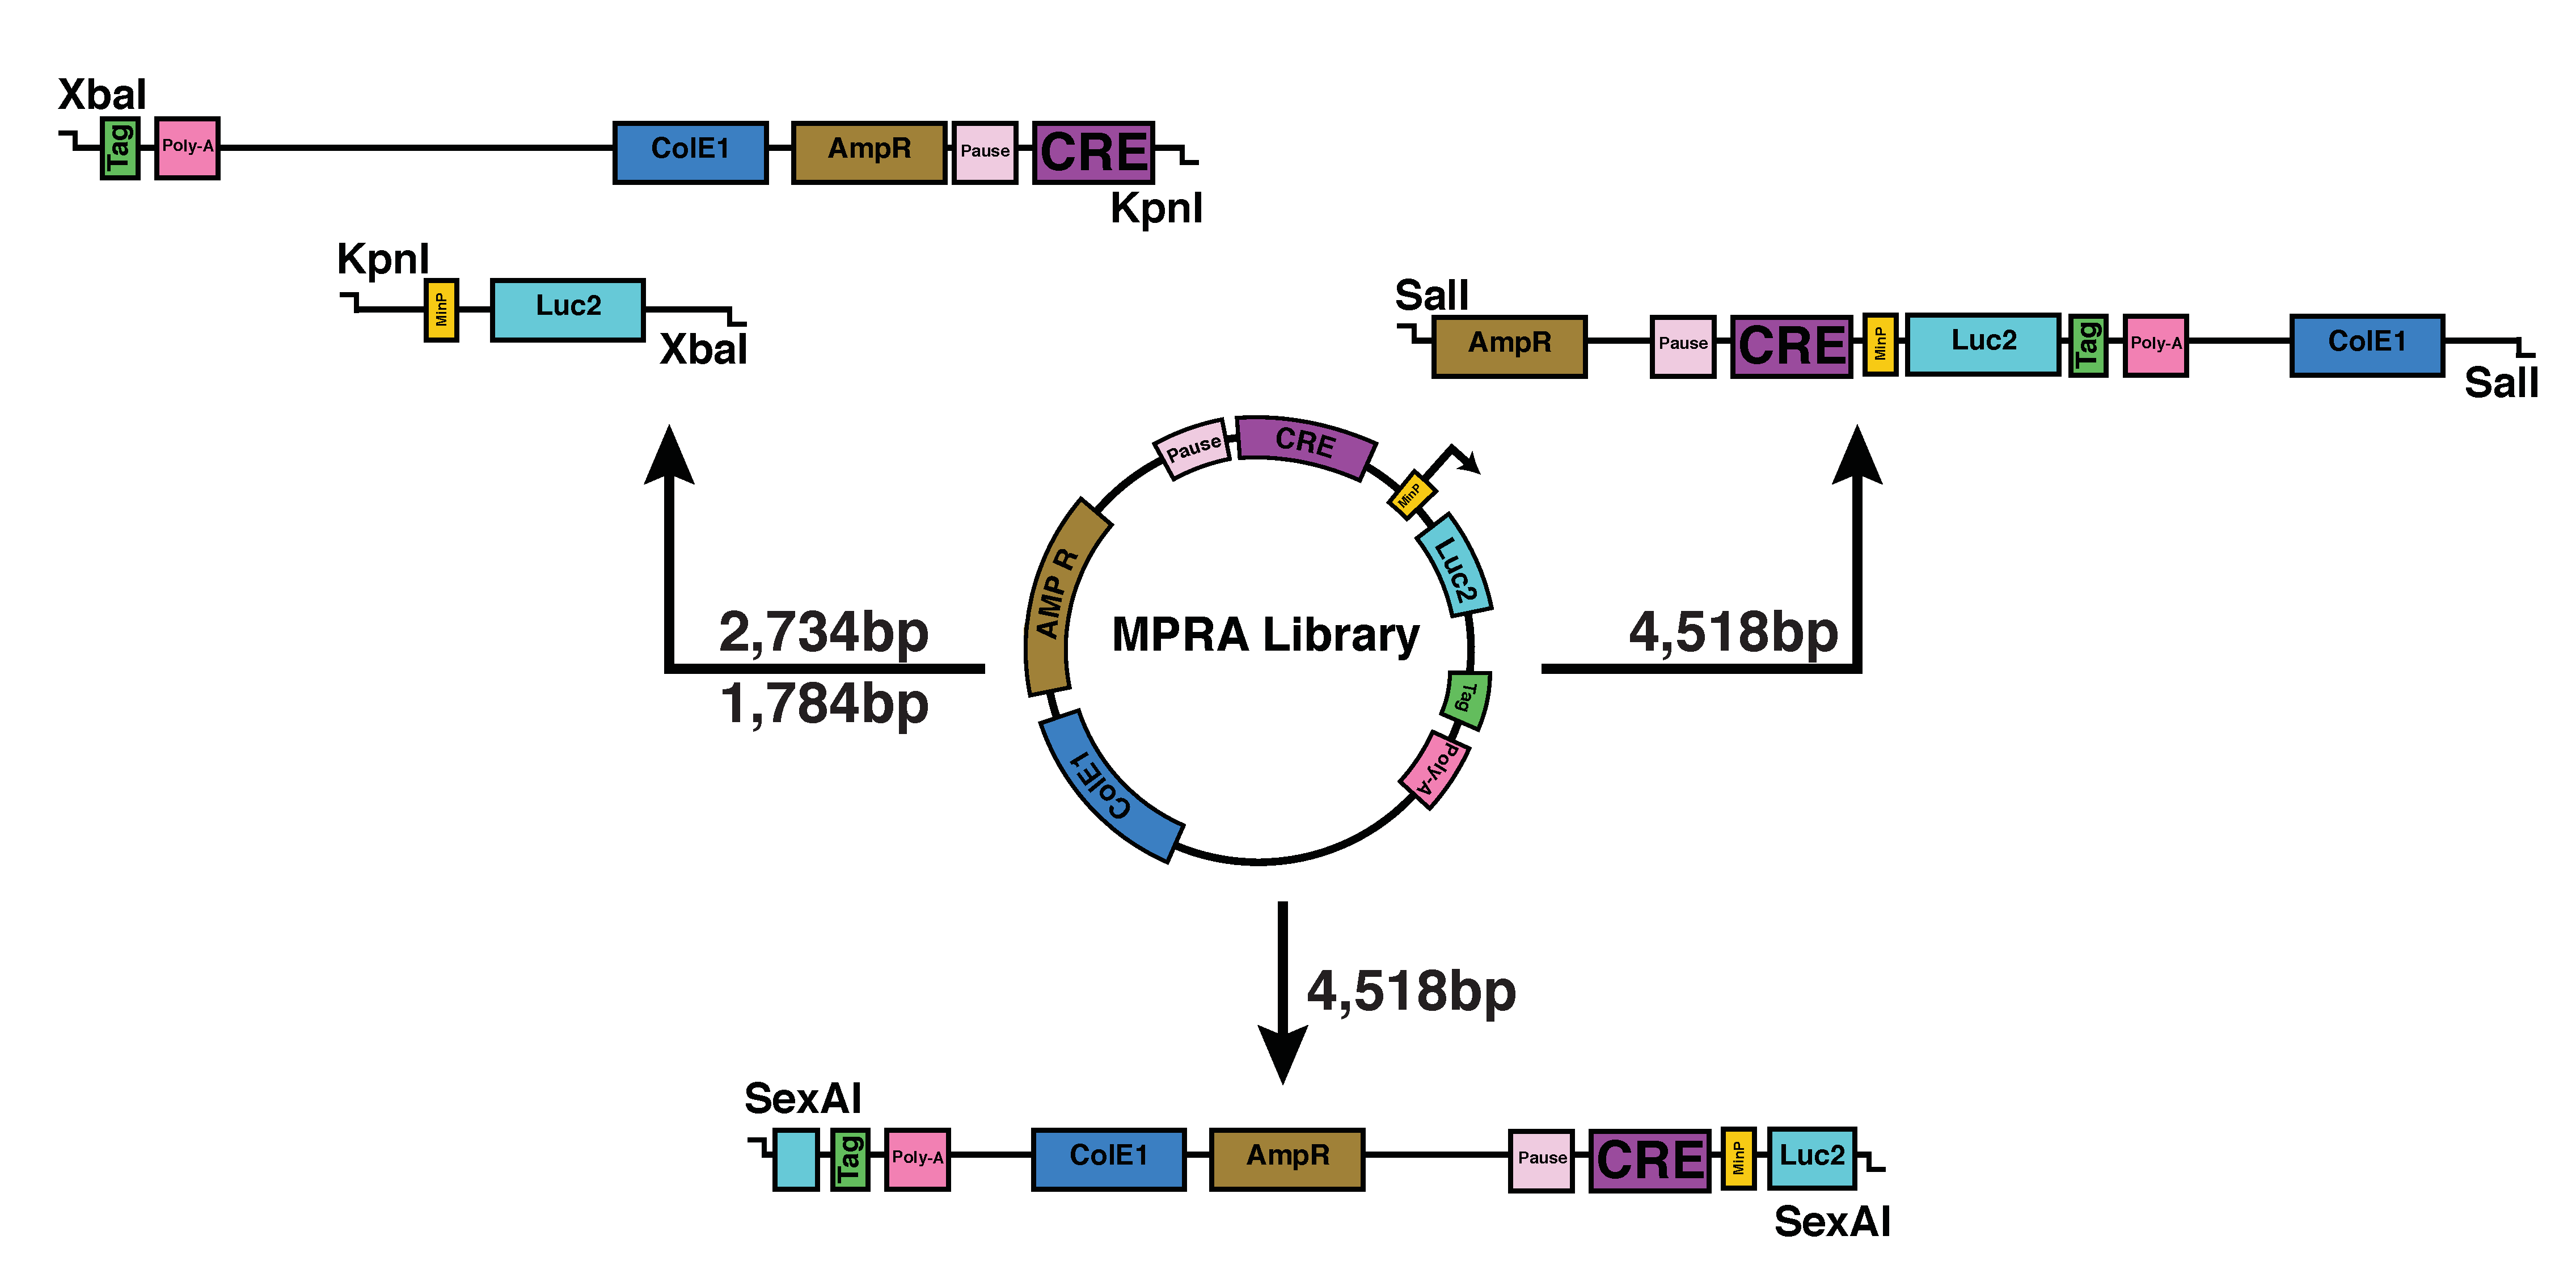
\includegraphics[width=1\textwidth]{CompetentLibDigest.pdf}
			\label{fig:CompLib_DigestFig}
			\caption{Competent Library QC Digest Expected Results}
        \end{figure}
        
        \begin{figure}[H]
			\centering
			\includegraphics[width=1\textwidth]{Comp_Lib_Digest.pdf}
			\label{fig:CompLib_Digestgel}
			\caption{Competent Library QC Digest Results}
        \end{figure}
        
        \begin{itemize}
		
        \item Nicked and super-coiled variants may escape digestion therefore they can be identified by running non-digested plasmid in an alternate lane. In Figure \ref{fig:CompLib_Digestgel} the super-coiled is around the same size as the backbone with MinP and Luciferase removed (\~2.7Kb) and SexAI appears to be low in activity. 
        
        \end{itemize}
        
	\subsection{Barcode Sequencing of Competent Library}
     	\begin{itemize}
     		
            \item PCR conditions for bar-code sequencing of competent library
 
		\end{itemize}
        
        \FloatBarrier
            \begin{table}[H]
				\centering
				\begin{tabular}{l|r|r}
					Reagent 					& 1x 				& 9x 				\\\hline
					2x NEB High Fidelity 		& 25\textmu L		& 225\textmu L		\\
					Library DNA(15ng/\textmu L) & 1\textmu L 		& 9\textmu L		\\
                    F+R-Primer (10uM) 			& 2.5\textmu L 		& 22.5\textmu L		\\                  
                    Water 						& 21.5\textmu L		& 193.5\textmu L		\\\hline
                    Final Volume 				& 50\textmu L 		& 450\textmu L
				\end{tabular}
           		\caption{\label{BCPCR}Volumes Barcode PCR Reactions.}
           \end{table}
           
        \FloatBarrier
            \begin{table}[H]
				\centering
				\begin{tabular}{l|r|r|r}
					Stage 	& 	Temperature	&	Time	&	Cycles		\\\hline
					Stage 1	&	98C			&	30 Sec.	&	1 Cycle		\\\hline
							&	98C			&	10 Sec.	&				\\
                    Stage 2	&	65C			&	30 Sec.	&	12 Cycles	\\
                    		&	72C			&	30 Sec.	&				\\\hline
                    Stage 3	&	72C			&	2 Min.	&	1 Cycle		\\
				\end{tabular}
           		\caption{\label{BarCodePCR}PCR Conditions for Barcode Amplification.}
           \end{table}
           
        \begin{itemize}
     		
            \item Purify with Qiagen min elute and check for target amplicon size around 131bp
            
            \item Check size on bioanalyzer high sensitivity DNA chip
            
        \end{itemize}
        
        \begin{figure}[H]
			\centering
			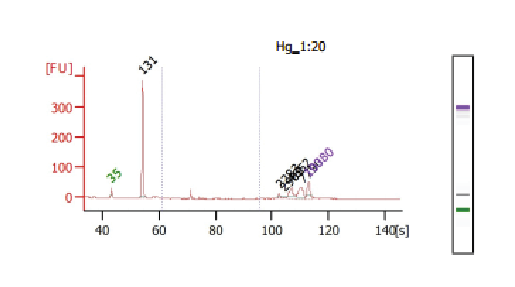
\includegraphics[width=1\textwidth]{BarcodeSeqTrace.pdf}
			\label{fig:BarcodeSize}
			\caption{Bar-code containing amplicons}
        \end{figure}
        
               
        \begin{itemize}
            
            \item Expected size with 5 degenerate bases on the 5' primer is 131 base pairs. Sequence amplicons 2x150bp
 
		\end{itemize}

\section{Competent Library Characterization}  

	\subsection{Library Activity}
    	\begin{itemize}
        
        	\item Four Co-Transfections for each condition were preformed at 2\textmu g of designated plasmid and 10ng of PGL 4.72 Renilla Luciferase per-2 million cells. One mL of media was added to each cuvette and 250\textmu L were plated per-well on a six well plate for 24hours.
            
            \item Luciferase assays were preformed with Promega Dual Luciferase Assays (	E1910) and read on a Promega Luminometer(GM3500) 
        
        \end{itemize}
    	 
        \begin{figure}[H]
			\centering
			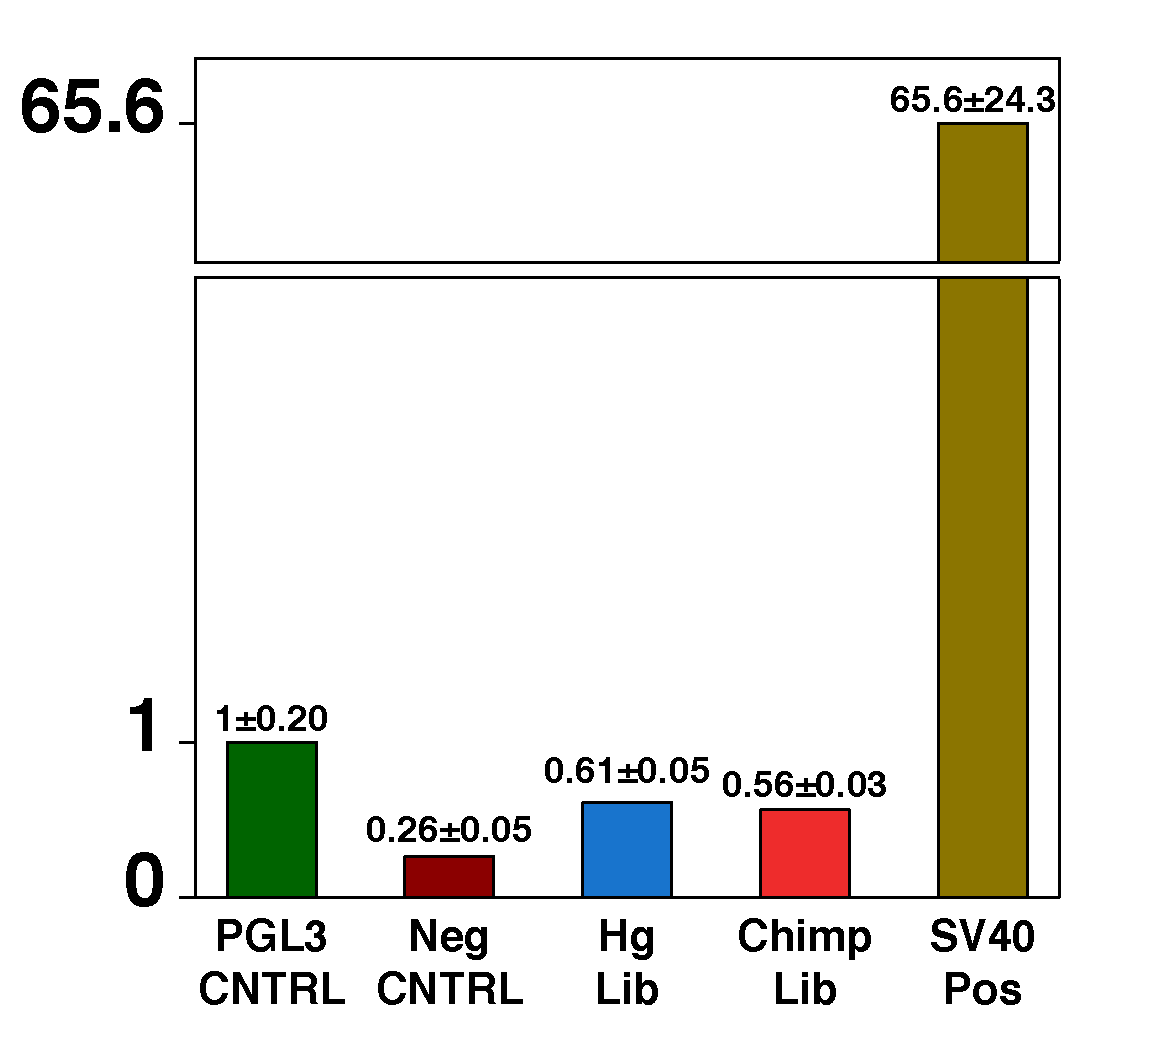
\includegraphics[width=1\textwidth]{2016_07_08_IndvLibs_VersusCNTRLsFINAL.pdf}
			\label{fig:Lib_Act}
			\caption{Competent Library Transfection}
        \end{figure}
    
    \subsection{Optimize Library Amount to Transfect}
    	\begin{itemize}
        
        	\item Libraries were C0-transfected with 2, 4, 8, and 16\textmu g of human plasmid library and 15ng of 4.72 Renilla Luciferase per-2 million cells. One mL of media was added to each cuvette and 250\textmu L were plated per-well on a six well plate for 24hours. 
            
            \item Luciferase assays were preformed with Promega Dual Luciferase Assays (	E1910) and read on a Promega Luminometer(GM3500) 
        
        \end{itemize}
    
   		\begin{figure}[H]
			\centering
			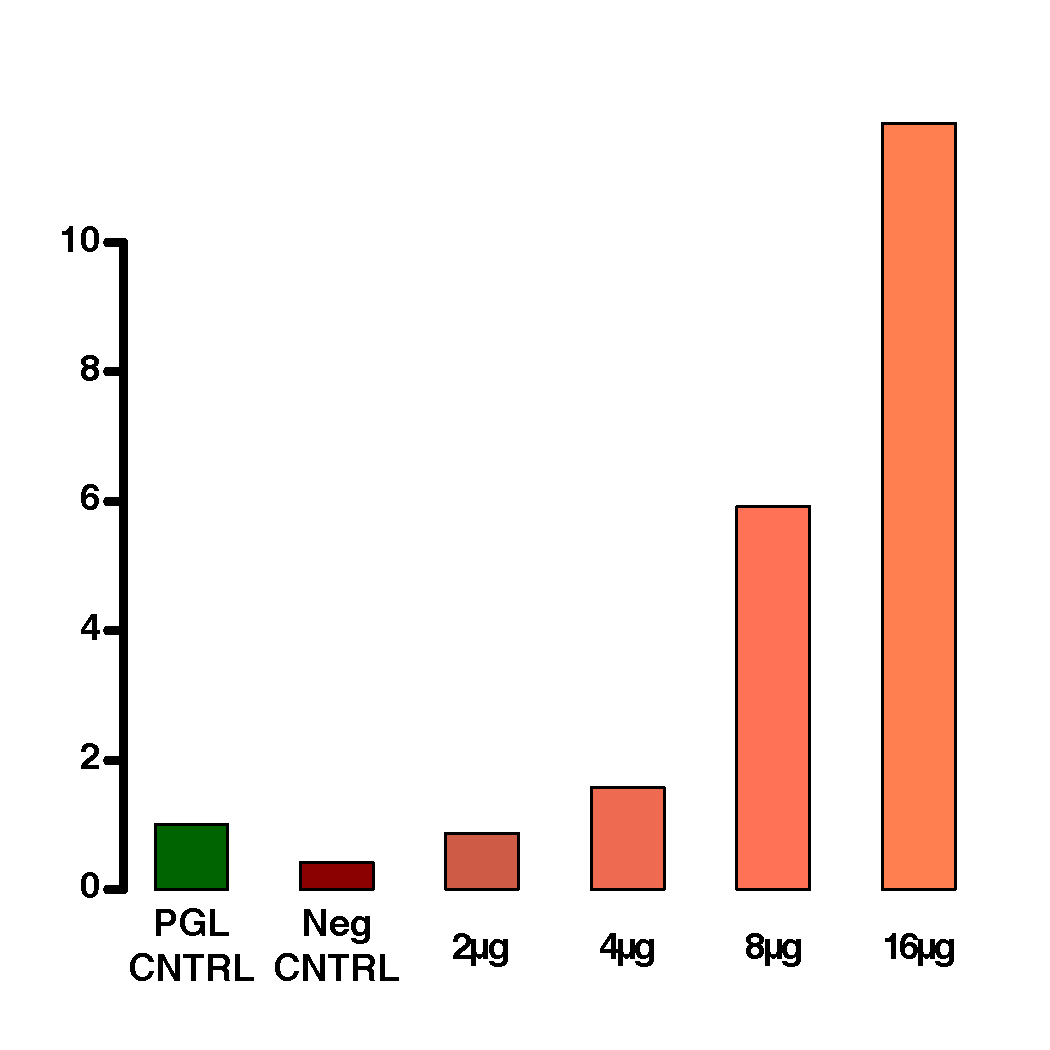
\includegraphics[width=1\textwidth]{2016_07_14_IncreasingLibraryFINAL.pdf}
			\label{fig:Lib_Amt}
			\caption{Transfection of Increasing Amounts of Library}
        \end{figure}
        
   	\subsection{Optimize Amount of Cells to Transfect}
		\begin{itemize}
        	\item Libraries were C0-transfected with 2, 4, 8, and 16 million cells, 16\textmu g plasmid library per- 2 million cells, and 20ng of 4.72 Renilla Luciferase per-2 million cells. One mL of media was added to each cuvette and 250\textmu L were plated per-well on a six well plate for 24hours. 
            
          	 \item Luciferase assays were preformed with Promega Dual Luciferase Assays (	E1910) and read on a Promega Luminometer(GM3500) 
        
        \end{itemize}
    
   		\begin{figure}[H]
			\centering
			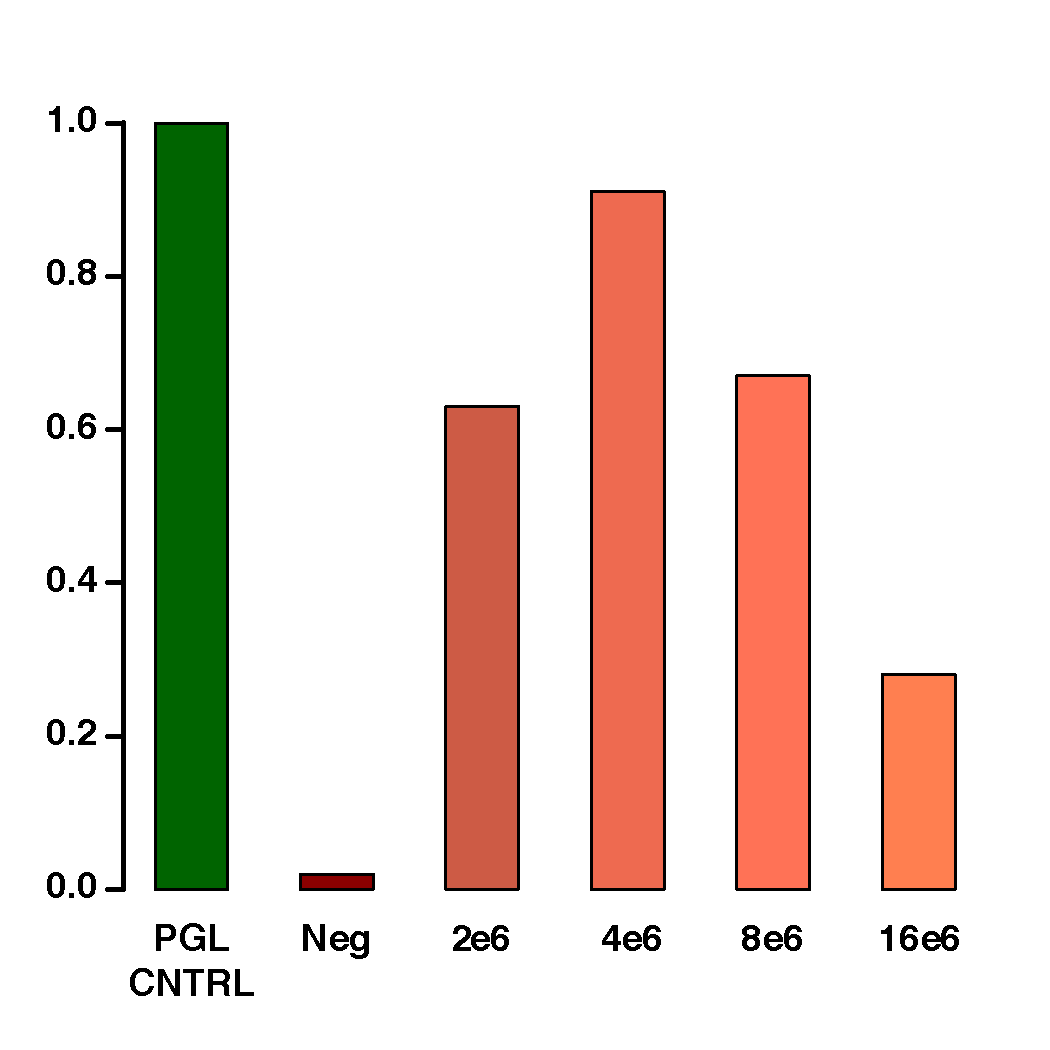
\includegraphics[width=1\textwidth]{2016_07_21_HC_diff_CellsFINAL.pdf}
			\label{fig:cell_Amt}
			\caption{Transfection of Increasing Amounts Cells}
        \end{figure}
		
        \begin{itemize}
        	\item Note: PGL Control seems extremely active here. Around 10 fold more active than previously, as evidence by extremely low negative control activity. 
        
        \end{itemize}
\section{Library Transfection}    
	\subsection{Harvest the cells}
    	\begin{itemize}
			
            \item Wash cells with 10mL (T-75) PBS (-) MgCl (-) CaCl, aspirate PBS
            
            \item Pipette 5mL pre-warmed Acutase into T-75 flask and incubate for 5 minutes at 37$^{\circ}$C
            
            \item Tap the flask to dislodge cells and neutralize with 6mL of complete media, pipette into a falcon tube and spin down cells at 200xg for 4 minutes
            
            \item Aspirate off fluid and re-suspend the pellet in 5-10mLs of complete media
        
        	\item Count cells to quantify concentration
            
        \end{itemize}
	\subsection{Transfection Conditions} \label{TransfectionConditions}
    	\begin{itemize}
			
            \item Pipette 40 Million cells a 10mL falcon tube and spin down at 200xg for 4 minutes
            
            \item Aspirate off media completely and pipette 320\textmu g of plasmid library on top of the cell pellet

            \item Add 1mL of Amaxa mNSC Reagent with Supplement 1 added and gently pipette to re-suspend the cells
                        
            \item Gently re-suspend the cell pellet and transfer to 10 Amaxa cuvettes
        
			\item Electroporate the sample using pre-defined protocol \textbf{A-033}, and immediately add 1mL of complete media to recover after each transfection
            
            \item Use the pipette provided by Amaxa to add recovered cells to a falcon tube
            
        \end{itemize}
    \subsection{Plating Transfected cells}
    	\begin{itemize}
			
            \item \textbf{Before Transfection}: Coat two 150$cm^2$ flasks each with 12mL of coating media and 1 aliquot of matrigel for 1hr - Over Night
            \item Wash with 20mL of PBS (-) MgCl, (-) CaCl, aspirate off, and add 30mL of growth media. Leave plate in cell incubator to equilibrate
            
            \item Add half of the pooled recovered cell volume to each equilibrated 150$cm^2$ flask and grow for 6 hours before harvesting
            
        \end{itemize}
    
\section{Post Transfection Processing}    
	
    \subsection{Harvest the cells}
    	\begin{itemize}
        	\item Wash cells with 20mL PBS (-) MgCl (-) CaCl, aspirate PBS
            
            \item Pipette 10mL pre-warmed Acutase into each 150$cm^2$ flask and incubate for 6 minutes at 37$^{\circ}$C
            
            \item Tap the dish to dislodge cells and neutralize with 12mL of complete media, pipette into a 50mL falcon tube and spin down cells at 200xg for 4 minutes
            
            \item Aspirate off fluid and re-suspend the pellet in 10mLs of PBS (-) MgCl (-) CaCl.
            
            \item Remove 5\% of the total volume and place into a 1.5mL eppendorf tube for plasmid library recovery
            
            \item Spin both the 10mL falcon tube and the eppendorf tube down at 200xg for 4 minutes
        
    	\end{itemize}
    
    
    \subsection{Genomic DNA Purification}\label{Genomic Purification}
    	\begin{itemize}
        	
            \item Add 40\textmu L 1M DTT per 1mL of RLT buffer and re-suspend pellet in 600\textmu L of RLT lysis buffer plus DTT per-10 Million cells transfected. Pipette to mix.
            
        	\item Aspirate off the PBS from the 1.5mL eppendorf tube and add 350\textmu L of previously prepared lysis buffer 
            
            \item Pipette to re-suspend the cells and vortex to vigorously to lyse cells
            
            \item Spin the eppendorf tube down and then add the entire volume to a Qiagen DNA/RNA 2 and 1 genomic DNA column
            
            \item Spin at 8150xg for 30 seconds. \textbf{Proceed to section \ref{RNA Purification} until instructed to return.}
            
            \item Wash column with 500$\mu$L of buffer AW1 and spin at 8150xg for 30 seconds
            
            \item Wash column with 500$\mu$L of buffer AW2 and spin at full speed for 2 minutes
            
            \item Place in 1.5mL eppendorf tube and Pipette 80$\mu$L of EB onto the column an incubate for one minute 
            
            \item Elute by spinning at 8150xg for 1 minute
            
            \item Pipette another 80$\mu$L of EB onto the column an incubate for one minute
            
            \item Elute a second time by spinning at 8150xg for 1 minute
            
        \end{itemize}
    
    
    
    \subsection{RNA Purification} \label{RNA Purification}
    	\begin{itemize}
        
        	\item Add 40\textmu L 1M DTT per 1mL of RLT buffer and re-suspend pellet in 600\textmu L of RLT lysis buffer plus DTT per-10 Million cells transfected. Pipette to mix. 
        
        	\item Vortex well and pipette the solution onto a QiaShredder column in increments of 600\textmu L per column. Spin at max speed for 2 minutes.
            
            \item Add one volume of 70\% EtOH to the flow through and pipette the combined solution onto an RNAeasy Column in increments of 650\textmu L. Spin 8500xg for 1 minute, this should equate to two spins per sample given this volume.
            
            \item Add 350\textmu L of RW1 buffer to the column and spin at 8500xg for 30s.
            
            \item Digest DNA on column by adding 10\textmu L pre-aliquoted DNAse I to 70\textmu L RDD buffer and pipetting all 80 \textmu L directly onto the column. Incubate at room temperature with lid closed for 15 minutes. \textbf{While the digesting DNA return to Section \label{Genomic Purification} and finish the genomic DNA purification}
            
            \item Add 350\textmu L of RW1 buffer to the column and spin at 8500xg for 30s.
            
            \item Add 500\textmu L of buffer RPE to the column and spin at for 30s.
            
            \item Add 500\textmu L of buffer RPE to the column and spin at for 2 minutes.
            
            \item Place column in new collection tube and spin at full speed for 1 minute to dry.
            
            \item Place column in another new collection tube and pipette 30\textmu L of RNAse free water directly onto the column wait one minute then spin at 8500xg 
        
        	 \item Pipette another 30\textmu L of RNAse free water directly onto the column wait one minute then spin at 8500xg
        
			\item Pool total RNA from the same transfections together and remove 2\textmu L aliquots of DNA for gel and nano-drop analysis        
        \end{itemize}
        
    \subsection{Second DNAse Treatment} \label{Second DNAse Treatment}
		\begin{itemize}
        	
            \item Prepare a second DNAse digestion as described in table \ref{DNASE}. Scale as necessary up to 200\textmu L, then split into different tubes.
            
        \end{itemize}
        
        \FloatBarrier
            \begin{table}[H]
				\centering
				\begin{tabular}{l|r|r}
					Reagent 		& 1x 				& 2x 			\\\hline
					RNA 			& Y\textmu L		& Y\textmu L	\\
					Water 			& X\textmu L 		& X\textmu L	\\
                    Buffer RDD 		& 10\textmu L 		& 20\textmu L	\\                  
                    DNAseI 			& 2.5\textmu L		& 5\textmu L	\\\hline
                    Final Volume 	& 100\textmu L 		& 200\textmu L
				\end{tabular}
           		\caption{\label{DNASE}Second DNAse Digestion Mix.}
           \end{table}
           
           \begin{itemize}
        	
            \item Incubate ad room temperature for 20 minutes
            
        \end{itemize}
    \subsection{Plasmid Library Enrichment from Purified DNA}
		\begin{itemize}
    		
            \item \textbf{Preform while second digest is occurring in Section \ref{Second DNAse Treatment}}
            
    		\item Add 300\textmu L ERC buffer to 20-100\textmu L of pDNA
        	
        	\item Add 10\textmu L NaOAC (3M). Votex to mix and spin down
        
        	\item Add total sample to QiaPrep Spin Miniprep column (27106). Spin at 17900xg for 1 minute
        
        	\item Add 500\textmu L of PB buffer to column and spin at 17900xg for 1 minute
        
        	\item Add 750\textmu L of PE buffer to column and spin at 17900xg for 1 minute
        
        	\item Transfer column to new tube and spin at 17900xg for 1 minute to dry column
        	
            \item Place in 1.5mL eppendorf tube and Pipette 30$\mu$L of EB onto the column an incubate for one minute 
            
            \item Elute enriched pDNA by spinning at 17900xg  for 1 minute
            
            \item Pipette another 30$\mu$L of EB onto the column an incubate for one minute
            
            \item Elute a second time by spinning at 8150xg for 1 minute
    
    \end{itemize}
    
    \subsection{RNA Clean-up}
    	\begin{itemize}
        	
        	\item Add 350\textmu L of RLT buffer for every 100\textmu L of DNAse treated RNA.
            
            \item Add 250\textmu L of 96-100\% RNAse free EtOH for every 100\textmu L of DNAse treated RNA.
            
            \item Pipette up to 700\textmu L onto an RNAeasy Mini-prep column and spin at 8500xg for 30s. Repeat as necessary up to column limit of 100\textmu g.
            
            \item Pipett 500\textmu L of RPE onto column and spin at 8500xg for 30s.
            
            \item Pipett 500\textmu L of RPE onto column and spin at 8500xg for 2 minutes.
        	
            \item Place column in new collection tube and spin at full speed for 1 minute to dry.
            
            \item Place column in another new collection tube and pipette 30\textmu L of RNAse free water directly onto the column wait one minute then spin at 8500xg 
        
        	 \item Pipette another 30\textmu L of RNAse free water directly onto the column wait one minute then spin at 8500xg
        
			\item Pool total RNA from the same transfections together and remove 2\textmu L aliquots of DNA for gel and nano-drop analysis        
        \end{itemize}
    \subsection{mRNA Purification (If Necessary)}
    	\begin{itemize}
			
        	\item Dilute 1-5\textmu g of total RNA to 50\textmu L with RNAse free water
            
            \item Pipette 20\textmu L of re-suspended beads in a \textbf{Separate Tube}
            
            \item Add 100\textmu L of binding buffer to the beads and mix by gently pipetting
            
            \item Place beads on Magnet for 2 minutes
            
            \item Remove supernatant, and then remove the tube from the rack and wash with another 100\textmu L of binding buffer mix gently by pipetting, 2 minutes magenet, remove supernatant, remove the tube from the rack.
            
            \item Re-suspend the beads in 50\textmu L binding buffer and then add 50\textmu L of total RNA, mix gently by pipetting
            
            \item Heat the entire reaction at 65$^{\circ}$C for 5 minutes and then hold at 4$^{\circ}$C or on ice for 3 minutes to denature secondary structure.
            
            \item Re-suspend beads gently by pipetting 
            
            \item Incubate at room temperature for five minutes.
            
            \item Re-suspend beads gently by pipetting 
            
            \item Incubate at room temperature for five minutes.
            
            \item Place tube on magnet for 2 minutes and discard the supernatant.
            
            \item Remove the tube from the rack and wash with 200\textmu L washing buffer, mix by pipetting then place the tube on the magnet for 2 minutes and discard the supernatant.
            
            \item Repeat the previous step a second time
            
            \item Re-suspend the beads in 50\textmu L of Tris, mix by pipetting and transfer to thin wall 0.2mL PCR tube.
            
            \item Heat sample in a thermocycler at 80$^{\circ}$C for 2 minutes, then hold at 25$^{\circ}$C to elute. Remove the samples when they reach 25$^{\circ}$C
            
            \item Add 50\textmu L binding buffer to each sample to allow the RNA to bind to the same beads. Mix by pipetting.
            
            \item Incubate at room temperature for five minutes.
            
            \item Re-suspend beads gently by pipetting 
            
            \item Incubate at room temperature for five minutes.
            
            \item Place tube on magnet for 2 minutes and discard the supernatant.
            
            \item Remove the tube from the rack and wash with 200\textmu L washing buffer, mix by pipetting then place the tube on the magnet for 2 minutes and discard the supernatant.
            
            \item Spin down tube then place back on magnet and remove the remaining supernatant with a 20\textmu L pipette
            
            \item Remove teh tube from the rack and re-suspend the beads in 17\textmu L of Tris, mix by pipetting and transfer to thin wall 0.2mL PCR tube.
            
             \item Heat sample in a thermocycler at 80$^{\circ}$C for 2 minutes, then hold at 25$^{\circ}$C to elute. Immediately remove the samples when they reach 25$^{\circ}$C and place on the magnetic rack for 2 minutes.
             
             \item Collect the enriched mRNA and remove 2\textmu L aliquots of DNA for gel and nano-drop analysis         
    	\end{itemize}
    \subsection{RNA QC}
    	\begin{itemize}
		
		\item Run an Agilent Eukaryotic RNA Pico chip with samples of 1:100 and 1:1000 dilutions of extracted and digested RNA. If mRNA enrichment was preformed run lanes of mRNA and a 1:10 dilution of mRNA.
        
		\end{itemize}
	\subsection{cDNA Synthesis}
    	\begin{itemize}
        
        	\item First Strand synthesis preformed with Invitrogen SSIII (18080-400). Reaction size scaled 2.5x as follows.
            
        \end{itemize}
            \FloatBarrier
            \begin{table}[H]
				\centering
				\begin{tabular}{l|r}
					Reagent & Volume \\\hline
					Annealing Buffer & 2.5\textmu L\\
					Oligo dt & 2.5\textmu L\\
                    mRNA & 15\textmu L\\\hline
                    Final Volume & 20\textmu L
				\end{tabular}
           		\caption{\label{Annealing}Volumes for a Single Oligo dt Annealing Reaction.}
           \end{table}
            
       \begin{itemize}
       		
       		\item Incubate 20\textmu L annealing reaction in DNAse/RNAse free PCR tube at 65C for 5 minutes then immediately place on ice
        	
            \item Add 2x buffer and SSIII enzyme to each reaction and incubate at 50C for 2.5 hours in a thermocycler with the lid set at 60C
           

		\end{itemize}
            \FloatBarrier
            \begin{table}[H]
				\centering
				\begin{tabular}{l|r}
					Reagent & Volume \\\hline
					Annealing Reaction & 20\textmu L\\
					2x Buffer & 25\textmu L\\
                    SSIII Enzyme & 5\textmu L\\\hline
                    Final Volume & 50\textmu L
				\end{tabular}
           		\caption{\label{Annealing}Volumes for a Single cDNA Synthesis Reaction.}
           \end{table}
	
    \subsection{cDNA Second Strand Synthesis}
		\begin{itemize}
        	
            \item Add DEPC treated water, 10x buffer, and enzyme mix (NEB E6111) to each reaction. Pipette 50\textmu L aliquots into 0.2mL PCR tubes and incubate at 16C for 2.5 hours in a thermocycler with the lid left unheated.
            
        \end{itemize}
		\begin{table}[H]
				\centering
				\begin{tabular}{l|r}
					Reagent & Volume \\\hline
					1st Strand Reaction & 50\textmu L\\
					DEPC Water & 120\textmu L\\
                    10x Buffer & 20\textmu L\\
                    Enzyme mix & 10\textmu L\\\hline
                    Final Volume & 200\textmu L
				\end{tabular}
           		\caption{\label{Annealing}Volumes for a Single cDNA Synthesis Reaction.}
           \end{table}
           \begin{itemize}
        	
            \item Clean up reactions with Qiagen Minelute columns, try to keep volume as minimal as possible to help in PCR amplification
                        
        \end{itemize}
\section{qPCR}
    	\subsection{Preparation}
		\begin{itemize}
        	
            \item Primer Stocks: All Primers are kept at 100uM, mix 10\textmu L forward with 10\textmu L reverse, and 80\textmu L for 100\textmu L of 10uM working stock
            
            \item Dilute 2\textmu L of cDNA 10-fold and 100-fold
            
            \item Dilute 2\textmu L of pDNA 10-fold, 100-fold, and 1,000-fold
            
            \item Serial dilute plasmid standard out fresh each time from $1\times10^8$copies/\textmu L to $1\times10^2$copies/\textmu L 
        \end{itemize}
	\subsection{Master Mix}
    	\begin{itemize}
        	
            \item All samples and standards are run in triplicate with an additional fourth reaction included to compensate for pipette error
            
            \item factor in 2-4 additional reactions into the master mix to account for pipette error as the master mix is very viscous
            
            \item Include a water and genomic DNA control as well
            
            \item Once total number of samples are accounted for make master mix as follows:
             
        \end{itemize}
        \begin{center}
        	
            $Samples_{total} = Samples\times4 + 4$
		\end{center}
        
    	\begin{table}[H]
				\centering
				\begin{tabular}{l|r|l|r}
					Reagent						&	Volume/Rxn			&	Scale to Volume					\\\hline
					2x Power Syber Master Mix	&	10\textmu L			&	$\times Samples_{total}$		\\
					DEPC Water					&	8\textmu L			&	$\times Samples_{total}$		\\
                    10uM F+R Primer Mix			&	1\textmu L			&	$\times Samples_{total}$		\\
                    Sample						&	1\textmu L			&	NA								\\\hline
                    Final Volume				&	20\textmu L			&	$19$\textmu L$\times Samples_{total}$
				\end{tabular}
           		\caption{\label{qPCR}qPCR Master Mix.}
       \end{table}
       \begin{itemize}

			\item Pipette 76\textmu L into each well along the D or E rows of a 96-well Fast Optical qPCR Plate (Applied Biosystems 4346906)

			\item Add 4\textmu L of sample to each well
            
            \item Use the multi-channel P200 pipette to pipette 20\textmu L of the 80\textmu L reaction into the three wells above (Row D) or below (Row E)
            
	   \end{itemize}

	\subsection{Sample qPCR Plate Layout}
		\begin{itemize}
        	
            \item Below is a sample qPCR plate layout
            
        \end{itemize}
        
        \begin{figure}[H]
			\centering
			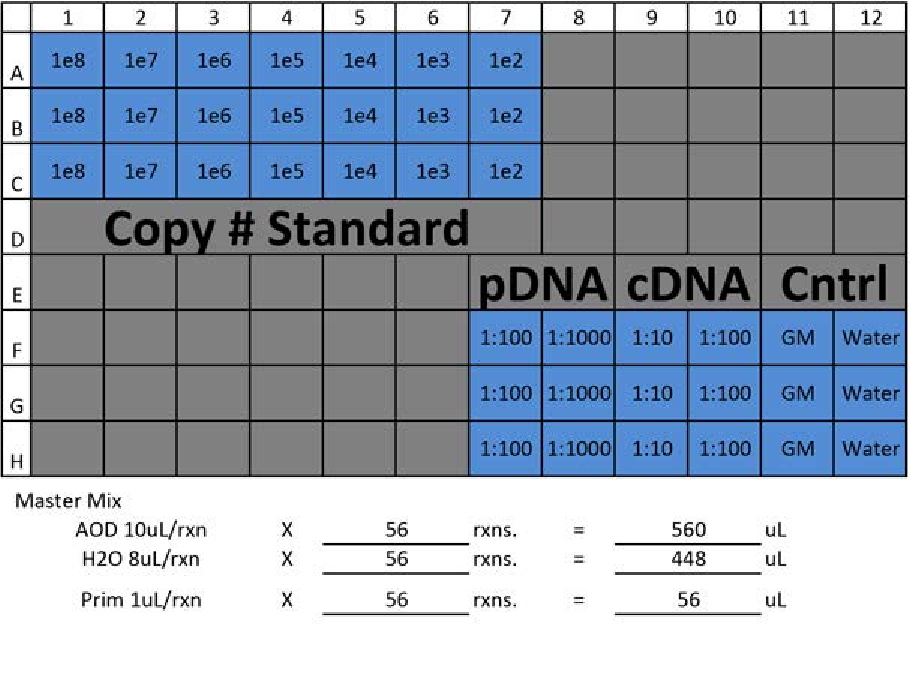
\includegraphics[width=1.0\textwidth]{qPCR_Template.pdf}
			\label{fig:qPCR_Template}
			\caption{Sample Layout of qPCR Plate}
		\end{figure}
        
    \subsection{Bar-code PCR Amplification}
    	\begin{itemize}
        
        	\item Generic PCR Master-Mix for Barcode-Seq:
        
        \end{itemize}
        \FloatBarrier
         \begin{table}[H]
			\centering
			\begin{tabular}{l|r|r}
					Reagent 									& 	Volume 			\\\hline
					2x NEB Master Mix 							& 	10\textmu L 	\\
					Water 										& 	x\textmu L		\\
                    Fwd + Rev Primers (10\textmu mol/\textmu L)	& 	1.25\textmu L	\\
                    DNA 										& 	x\textmu L		\\\hline
                    Final Volume 								& 	20\textmu L		\\
				\end{tabular}
           		\caption{\label{BC_PCR}Barcode PCR Master-mix.}
        \end{table}     
        \begin{itemize}
        
        	\item Generic PCR Conditions for Barcode-Seq:
        
        \end{itemize}
        \FloatBarrier
            \begin{table}[H]
				\centering
				\begin{tabular}{l|r|r|r}
					Stage 	& 	Temperature	&	Time	&	Cycles		\\\hline
					Stage 1	&	98C			&	30 Sec.	&	1 Cycle		\\\hline
							&	98C			&	10 Sec.	&				\\
                    Stage 2	&	65C			&	20 Sec.	&	X Cycles	\\
                    		&	72C			&	30 Sec.	&				\\\hline
                    Stage 3	&	72C			&	2 Min.	&	1 Cycle		\\
				\end{tabular}
           		\caption{\label{BC_PCR}PCR Conditions for Sample Barcode Amplification.}
           \end{table}
           
           \begin{itemize}
        
        	\item Before you can amplify the cDNA or pDNA fractions for sequencing you need to figure out the optimal amount of PCR cycles for however many template copies you want to seed for each 20 \textmu L PCR reaction.
            
            \item Observation of amplification per-cycle (for 40 cycles) of the 1:10 dilutions with SYBR green under  actual PCR conditions is needed as follows:
        
        \end{itemize}
         \FloatBarrier
         \begin{table}[H]
			\centering
			\begin{tabular}{l|r|r}
					Reagent 									& 	Volume 			\\\hline
					2x NEB Master Mix 							& 	10\textmu L 	\\
					Water 										& 	6.55\textmu L	\\
                    Fwd + Rev Primers (10\textmu mol/\textmu L)	& 	1.25\textmu L	\\
                    10x SYBR Green								&	1.2 \textmu L 	\\
                    DNA 										& 	1\textmu L		\\\hline
                    Final Volume 								& 	20\textmu L		\\
				\end{tabular}
           		\caption{\label{BC_PCR}Barcode qPCR Master-mix.}
        \end{table} 
        
        
   		\begin{figure}[H]
			\centering
			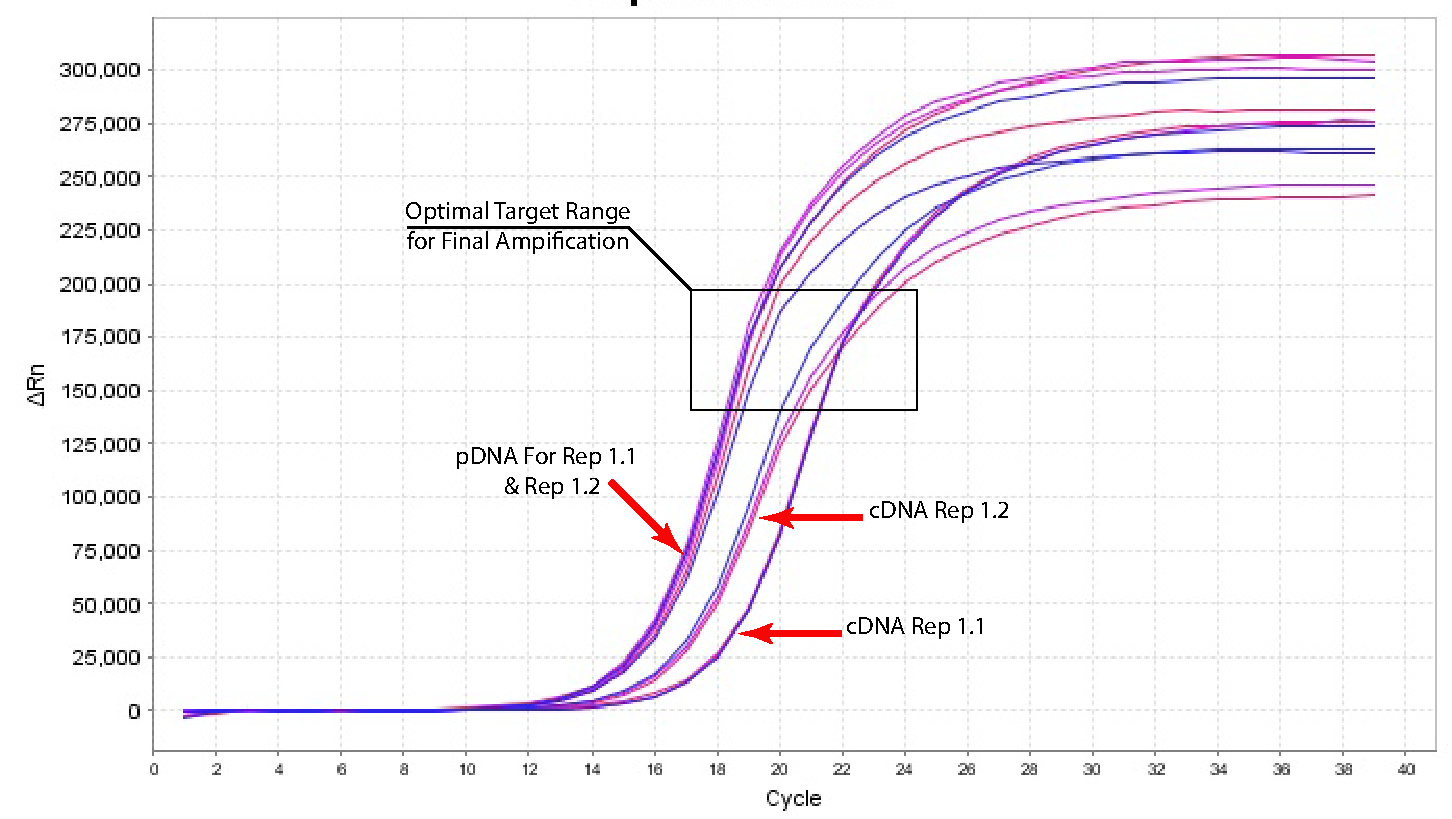
\includegraphics[width=1\textwidth]{2016_10_09_BarcodeSeq_qPCR_A_Fig.pdf}
			\label{fig:Sample_SYBR}
			\caption{SYBR Green Amplifiation}
        \end{figure}
        \begin{itemize}
        
        	\item Repeat Amplification with undiluted pDNA. Take the cycle number around the desired range and subtract four cycles for the dilution change. Round up, and add one cycle to be safe. In the case of Figure \ref{fig:Sample_SYBR} 15 cycles seems sufficient. 
        
        \end{itemize}
        \begin{figure}[H]
			\centering
			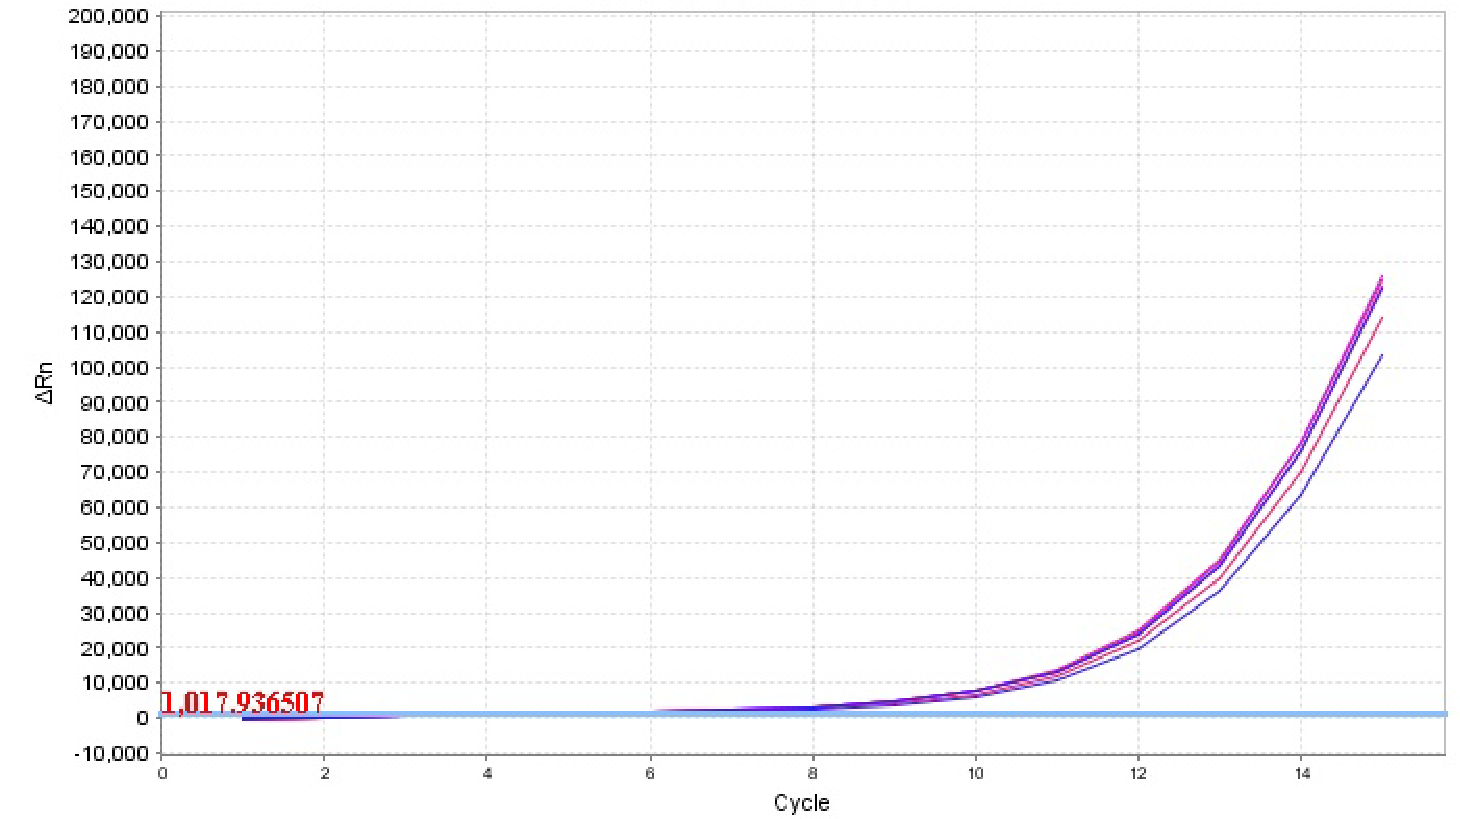
\includegraphics[width=1\textwidth]{2016_10_09_BarcodeSeq_1uL_pDNA_reps1_1_1_2_jpg.pdf}
			\label{fig:SYBR_pDNA}
			\caption{pDNA Undiluted SYBR Green Amplifiation}
        \end{figure}
        \begin{itemize}
        
        	\item Figure \ref{fig:SYBR_pDNA} is just on the lower end of optimal, but will work. 
        	
            \item Next step is to run out wells from both SYBR reactions on a 2\% Agarose gel and then purify seperate wells with a Qiagen minelute column and run them on an Agilent DNA High Sensitivity chip. This will confirm that there are no off target effects and also that there will be enough product produced at the flourescent intensity in Figure \ref{fig:SYBR_pDNA}.
        
        \item Generic PCR Conditions for pDNA Barcode-Seq:
        
        \FloatBarrier
            \begin{table}[H]
				\centering
				\begin{tabular}{l|r|r|r}
					Stage 	& 	Temperature	&	Time	&	Cycles		\\\hline
					Stage 1	&	98C			&	30 Sec.	&	1 Cycle		\\\hline
							&	98C			&	10 Sec.	&				\\
                    Stage 2	&	65C			&	20 Sec.	&	17 Cycles	\\
                    		&	72C			&	30 Sec.	&				\\\hline
                    Stage 3	&	72C			&	2 Min.	&	1 Cycle		\\
				\end{tabular}
           		\caption{\label{BC_PCR}PCR Conditions for Sample Barcode Amplification.}
           \end{table}
           
           \item Generic PCR Conditions for cDNA Barcode-Seq:
        
        \FloatBarrier
            \begin{table}[H]
				\centering
				\begin{tabular}{l|r|r|r}
					Stage 	& 	Temperature	&	Time	&	Cycles		\\\hline
					Stage 1	&	98C			&	30 Sec.	&	1 Cycle		\\\hline
							&	98C			&	10 Sec.	&				\\
                    Stage 2	&	65C			&	20 Sec.	&	18 Cycles	\\
                    		&	72C			&	30 Sec.	&				\\\hline
                    Stage 3	&	72C			&	2 Min.	&	1 Cycle		\\
				\end{tabular}
           		\caption{\label{BC_PCR}PCR Conditions for Sample Barcode Amplification.}
           \end{table}
           
	\end{itemize}
        
\section{Reagents}
    \subsection{Consumables}
    	\FloatBarrier
            \begin{table}[H]
				\centering
				\begin{tabular}{l|l|l}
Provider	&	Reagent	&	Product Number	\\\hline
American Bio	&	DEPC Water:AB02128-00500	\\
NEB	&	High Fiedelity 2x Master Mix	&	M0541L	\\
Life Technologies	&	SYBR Green	&	S7563	\\
Beckman Coulter	&	AMPureXP SPRI Beads	&	A63880	\\
NEB	&	BSA (20mg/mL)	&	B9000S	\\
NEB	&	Q5 High fidelity Polymerase	&	M0491L	\\
Acros Organics:2-Butanol	&	10770-0010	\\
Sage Science	&	2\% Agarose pippen prep gels	&	CSD2010	\\
NEB	&	CIP	&	M0290L	\\
NEB	&	400U/textmu L DNA T4 Ligase	&	M0202M	\\
American Bio	&	70\% Ethanol	&	AB04010-00500	\\
American Bio	&	200 Proof Ethanol	&	AB00515-00500	\\
Recombinant Thecnologies	&	100textmu g/mL LB/Amp plates	&	Stockroom	\\
Bio-Rad	&	Electroportion Cuvettes 0.1cm	&	1652089	\\
American Bio	&	Agarose	&	AB00972-00500	\\
Sigma	&	Ethidium Bromide	&	E1510-10ML	\\
American Bioanalytical	&	DMSO	&	AB03091-00100	\\
NEB	&	dNTPs	&	N0446S	\\
Promega	&	PGL 4.72 Renilla Luciferase Vector	&	E690A	\\
Promega	&	PGL 3 Control Vector	&	E174A	\\
Gibco	&	PBS Mg/Cl -	&	14190-144	\\
Gibco	&	StemPro Acutase	&	A11105-01	\\
Qiagen	&	DNAseI	&	79254	\\
American Bio	&	3M NaOAC	&	AB13168-01000	\\
ThermoFischerScientific	&	MegaX DH10B	&	C6400-03	\\
Applied Biosystems	&	Fast Optical qPCR Plates	&	4346906	\\
            \end{tabular}
           		\caption{\label{CReagents}Primary Consumable Reagents.}
           \end{table}
        
    \subsection{Kits}
    	\FloatBarrier
            \begin{table}[H]
				\centering
				\begin{tabular}{l|l|l}
             Provider	&	Kit	&	Product Number	\\\hline
CHIMERx/EURx	&	Micellula Emulsion PCR Kit	&	3600-02\\
Agilent	&	Bioanalyzer Eukaryotic Pico Kit	&	5067-1513\\
Agilent	&	Bioanalyzer High Sensitivity DNA	&	5067-4626\\
Qiagen	&	Minelute	&	28004\\
Qiagen	&	Reaction Clean-up (ERC Buffer is in here)	&	28206\\
Qiagen	&	HiSpeed Maxi Kit	&	12662\\
Qiagen	&	Endofree Mega Kit	&	12381\\
Qiagen	&	QiaShredder	&	79654\\
Qiagen	&	RNeasy Mini Kit	&	74104\\
NEB	&	NEBNext Library Kit	&	E6040L\\
NEB	&	HighSeq Indexing Primers	&	E7335L\\
Promega	&	Dual Luciferase Assay Kit	&	E1910\\
Qiagen	&	AllPrep Mini DNA/RNA	&	80204\\
Invitrogen	&	Super Script III cDNA kit	&	18080-400\\
             
             \end{tabular}
           		\caption{\label{KReagents}Primary Kit Reagents.}
           \end{table}
    \subsection{Specialized Equipment}
    	\begin{itemize}
        	\item Bio-Rad Gene Pulser
    		\item Amaxa Nucleofector 
            \item Applied Biosystems Step One Plus qPCR
            \item Agilent 2100 Bioanalyzer
            \item Promega Luminometer GM3500
    	\end{itemize}
\section{Primer Sequences}
	\subsection{Initial Low Cycle Library Primers}
    	
        \begin{itemize}
        
        	\item Forward: 5' - GCCAGAACATTTCTCT - 3'
            \item Reverse: 5' - GCAGGAGCCGCAGTG - 3'
        
        \end{itemize}      
   	
    \subsection{Library Bar-coding Primers}
    	
        \begin{itemize}
            
            \item Forward:5' \tiny{GCCAGAACATTTCTCTGGCCTAACTGGCCGCTTGACG} \normalsize{3'
          	\item Reverse:5'} \tiny{CCGACTAGCTTGGCCGCCGAGGCCCGACGCTCTTCCGATCTNNNNNNNNNNNNNNNNTCTAGAGGTACCGCAGGAGCCGCAGTG} \normalsize{3'}       
            
		\end{itemize}
        
   	\subsection{Inert TagSeq Library Primers}
        \begin{itemize}

			\item Forward:5' - (N:25252525)(N)(N)(N)(N)CAGGTGCCAGAACATTTCTCT  - 3'
        	\item Reverse:5' - TTATCATGTCTGCTCGAAGCGG - 3'
		        
        \end{itemize}
   \subsection{Competent TagSeq Primer}
        \begin{itemize}    
        	\item The 3' primer falls down of custom cDNA primer, allows for longer PCR product
            \item Forward:5' -(N:25252525)(N)(N)(N)(N)CAAGAAGGGCGGCAAGAT - 3'
        	\item Reverse:5' - TTATCATGTCTGCTCGAAGCGG - 3'
            
        \end{itemize}
   \subsection{Barcode-Seq  Primers: Targets cDNA}
        \begin{itemize}
			\item The 3' primer falls upstream of custom cDNA primer!!
			\item Forward:5' -(N:25252525)(N)(N)(N)(N)CGAGGTGCCTAAAGGACTG- 3'
        	\item Reverse:5' - CCGACGCTCTTCCGATCT - 3'
		        
 		\end{itemize}
   
   \subsection{Reverse Transcription Primer}
        \begin{itemize}

			\item 5' -CCGACTAGCTTGGCCGC- 3'
        	    
 		\end{itemize}
	
    \subsection{Transcript qPCR  Primers: targets Luciferase}
        \begin{itemize}

			\item Forward:5' -AACACCCCAACATCTTCGAC- 3'
        	\item Reverse:5' -TCTCGGTCATGGTTTTACCG- 3'
		        
 		\end{itemize}

	\subsection{Backbone qPCR  Primers}
        \begin{itemize}

			\item Forward:5' -ATTTGGTATCTGCGCTCTGC- 3'
        	\item Reverse:5' -TTTGCCGGATCAAGAGCTAC- 3'
		        
 		\end{itemize}
%\begin{enumerate}
%\item Like this,
%\item and like this.
%\end{enumerate}
%\dots or bullet points \dots
%\begin{itemize}
%\item Like this,
%\item and like this.
%\end{itemize}
%\dots or with words and descriptions \dots
%\begin{description}
%\item[Word] Definition
%\item[Concept] Explanation
%\item[Idea] Text
%\end{description}


\end{document}